%%%%%%%%%%%%%%%%%%%%%%%%%%%%%%%%%%%%%%%%%%  不使用 authblk 包制作标题  %%%%%%%%%%%%%%%%%%%%%%%%%%%%%%%%%%%%%%%%%%%%%%
%-------------------------------PPT Title-------------------------------------
\title{化学键的本质与生化反应动力学模拟}
%-----------------------------------------------------------------------------
%----------------------------Author & Date------------------------------------

%\author[\textrm{Jun\_Jiang}]{姜\;\;骏\inst{}} %[]{} (optional, use only with lots of authors)
%% - Give the names in the same order as the appear in the paper.
%% - Use the \inst{?} command only if the authors have different
%%   affiliation.
\institute[BCC]{\inst{}%
%\institute[Gain~Strong]{\inst{}%
\vskip -20pt 北京市计算中心~智能计算事业部}
%\vskip -20pt {\large 格致斯创~科技}}
\date[\today] % (optional, should be abbreviation of conference name)
{%	{\fontsize{6.2pt}{4.2pt}\selectfont{\textcolor{blue}{E-mail:~}\url{jiangjun@bcc.ac.cn}}}
\vskip 45 pt {\fontsize{8.2pt}{6.2pt}\selectfont{%清华大学\;\;物理系% 报告地点
%	\vskip 5 pt \textrm{2023.06}}}
%	\vskip 5 pt \textrm{2024.04.25}}}
	\vskip 5 pt \textrm{2024.07.24}}}
}

%% - Either use conference name or its abbreviation
%% - Not really information to the audience, more for people (including
%%   yourself) who are reading the slides onlin%%   yourself) who are reading the slides onlin%%   yourself) who are reading the slides onlineee
%%%%%%%%%%%%%%%%%%%%%%%%%%%%%%%%%%%%%%%%%%%%%%%%%%%%%%%%%%%%%%%%%%%%%%%%%%%%%%%%%%%%%%%%%%%%%%%%%%%%%%%%%%%%%%%%%%%%%

\subject{}
% This is only inserted into the PDF information catalog. Can be left
% out.
%\maketitle
\frame
{
%	\frametitle{\fontsize{9.5pt}{5.2pt}\selectfont{\textcolor{orange}{“高通量并发式材料计算算法与软件”年度检查}}}
\titlepage
}
%-----------------------------------------------------------------------------

%------------------------------------------------------------------------------列出全文 outline ---------------------------------------------------------------------------------
\section*{}
\frame[allowframebreaks]
{
  \frametitle{Outline}
%  \frametitle{\textcolor{mycolor}{\secname}}
  \tableofcontents%[current,currentsection,currentsubsection]
}
%%在每个section之前列出全部Outline
%%类似的在每个subsection之前列出全部Outline是\AtBeginSubsection[]
%\AtBeginSection[]
%{
%  \frame<handout:0>%[allowframebreaks]
%  {
%    \frametitle{Outline}
%%全部Outline中,本部分加亮
%    \tableofcontents[current,currentsection]
%  }
%}

%-----------------------------------------------PPT main Body------------------------------------------------------------------------------------
\small
\section{分子间相互作用与化学键}
%\frame
%
%	\frametitle{\textrm{VASP}计算的特色}
%	相比于与普通的第一原理计算软件,\textrm{VASP}很好地平衡了计算效率和精度的问题,总的来说,\textrm{VASP}主要通过这几个特色保证了计算的高效能
%	\begin{itemize}
%	     \item 迭代与优化算法的多样性\\
%		     本质上电荷密度迭代 \textrm{\&\&} 体系总能量优化是相同的优化问题,采用了类似的算法\upcite{CMS6-15_1996,PRB54-11169_1996}:\\
%			\textcolor{blue}{\textrm{Pseudo-Newton、Conjugate-Gradient、Broyden~mix、damping-factor、RMM-DIIS}}
%	     \item 尽可能采用局域基(原子轨道基)函数:~\\
%		     \textcolor{blue}{\textrm{LREAL}}=\textcolor{red}{\textrm{.TRUE.}}\\
%			优化的投影函数也尽可能在实空间表示
%	     \item \textrm{PAW}原子数据集:\textcolor{blue}{优异的赝势}\upcite{PRB59-1758_1999}
%	\end{itemize}
%}
\frame
{
	\frametitle{遗传学、分子生物学与生物化学}
\begin{figure}[h!]
\centering
\vspace{-5.5pt}
%\caption{\textrm{The wave-particle duality and Photoelectric effect}}
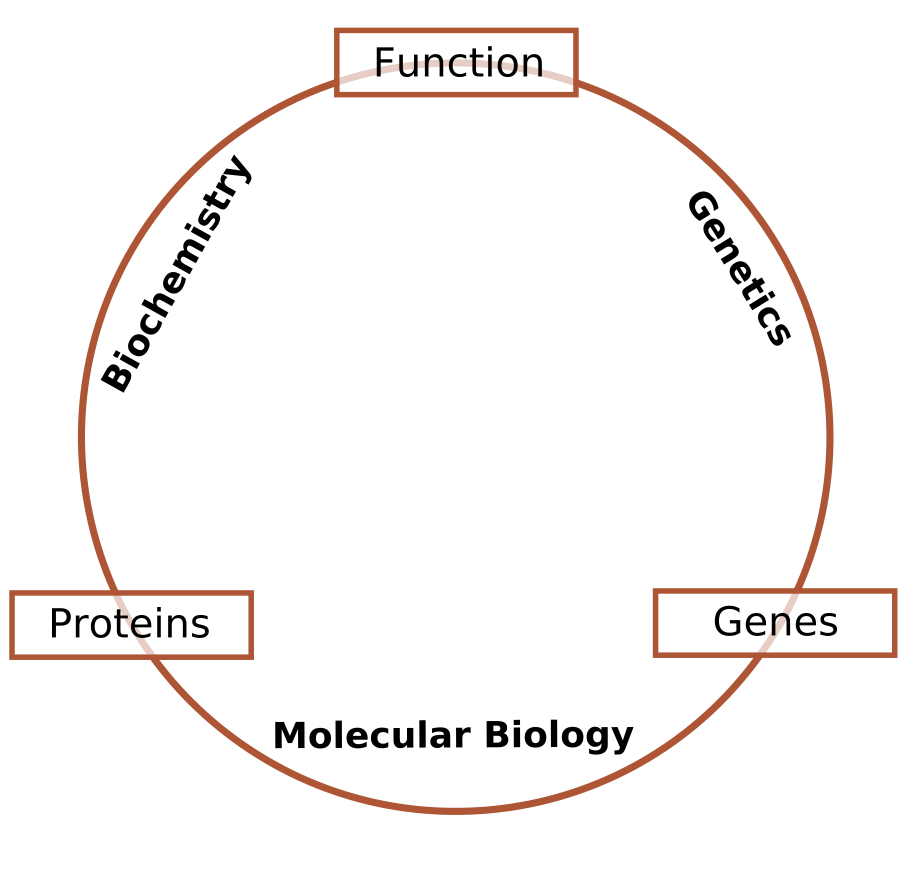
\includegraphics[height=2.80in,width=2.97in,viewport=0 0 720 680,clip]{Figures/Schematic_relationship_between_biochemistry_genetics_and_molecular_biology.png}
\label{Bio-Chem-Genetics}
\end{figure}
}

\frame
{
	\frametitle{生物化学反应的特点}
\begin{figure}[h!]
\centering
\vspace{-10.5pt}
%\caption{\textrm{The wave-particle duality and Photoelectric effect}}
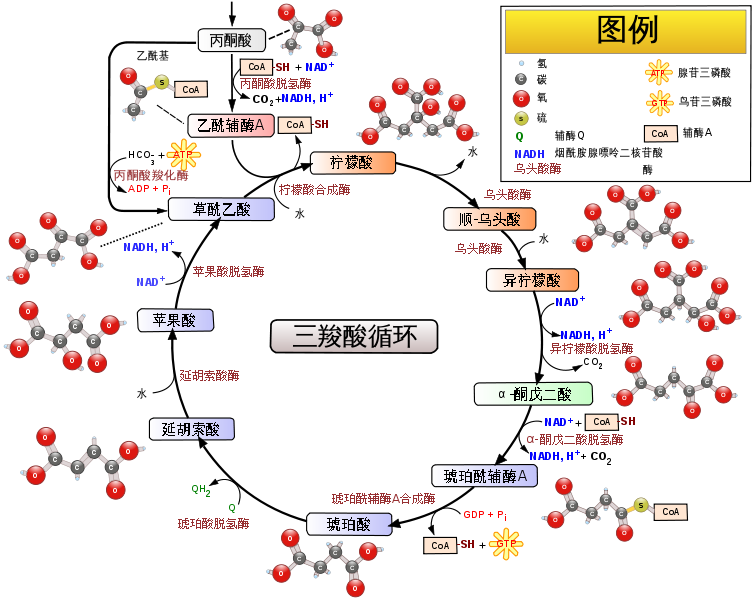
\includegraphics[height=2.80in,width=3.70in,viewport=0 0 750 600,clip]{Figures/Citric_acid_cycle_with_aconitate_Chinese.png}
\label{Bio-Chem}
\end{figure}
}

\frame
{
	\frametitle{生物化学反应机理研究}
\begin{figure}[h!]
\centering
\vspace{-8.5pt}
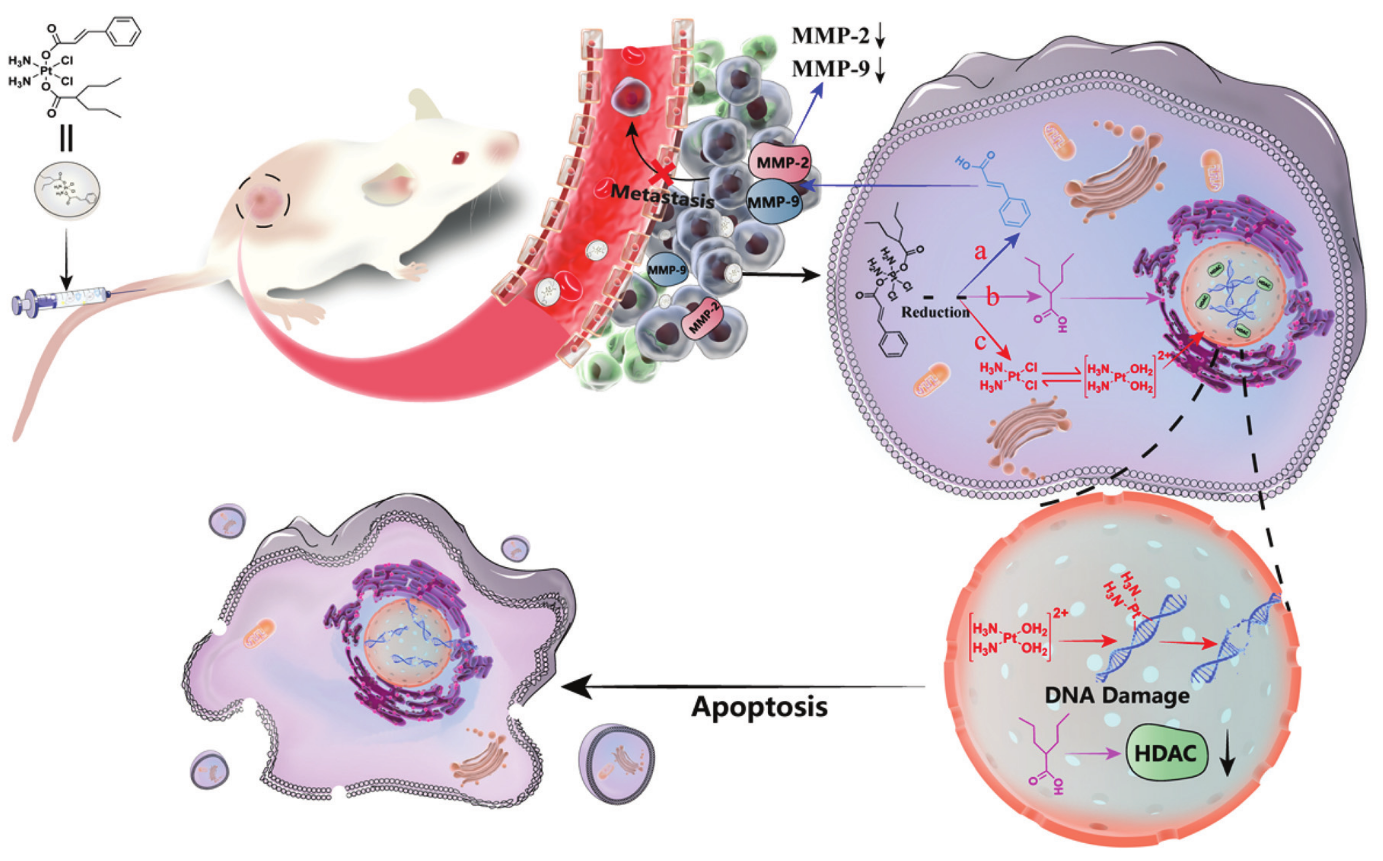
\includegraphics[height=0.67\textwidth,width=1.0\textwidth,viewport=0 0 1380 900,clip]{Figures/anti-tumour_mechanism-of the-Cin-Pt(IV)-Val-complex.png}
%\caption{\textrm{ABINIT}的Si.in}
\label{mechanism}
\end{figure}
}

\frame
{
	\frametitle{分子间相互作用与化学键}
\begin{figure}[h!]
\centering
\vspace{-25.5pt}
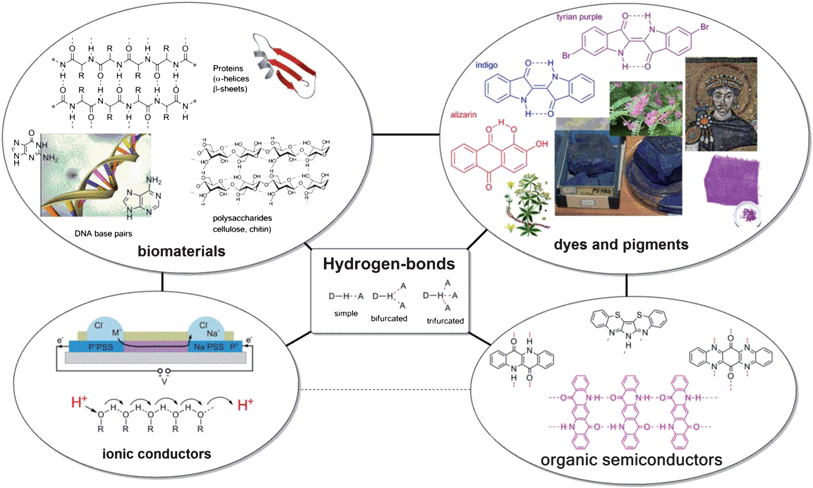
\includegraphics[height=0.67\textwidth,width=1.0\textwidth,viewport=0 0 830 500,clip]{Figures/Bio-H-bond-1.png}
%\caption{\textrm{ABINIT}的Si.in}
\label{Bio-H-bond}
\end{figure}
}

\frame
{
	\frametitle{微观相互作用的强度与分类}
\begin{figure}[h!]
\centering
\vspace{-5.5pt}
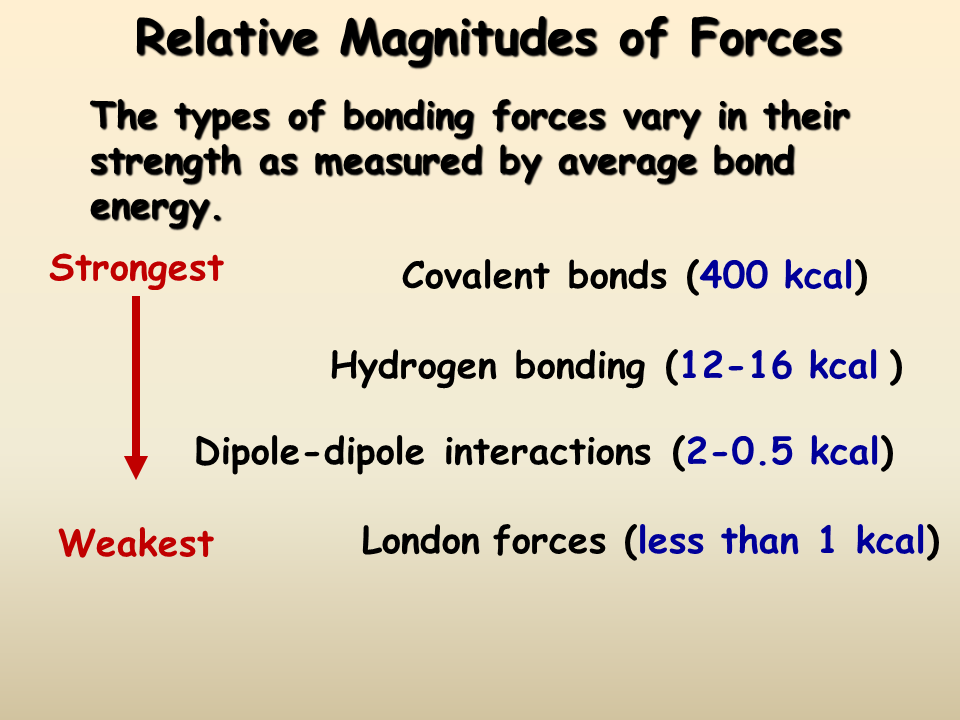
\includegraphics[height=0.65\textwidth,width=1.05\textwidth,viewport=0 100 750 530,clip]{Figures/Bond-order.png}
%\caption{\textrm{ABINIT}的Si.in}
\label{Bond-order}
\end{figure}
%{\centering\textcolor{magenta}{对化学键本质的认知:~时代呼唤量子力学}}
}

\subsection{蛋白质分子结构与活性位点}
\frame
{
	\frametitle{蛋白质的结构与分子间作用力}
\textcolor{blue}{质点运动发生在一个几何空间里,所以力学可以看成是某个几何空间里的动力系统}
\begin{figure}[h!]
\centering
\vspace{-40.5pt}
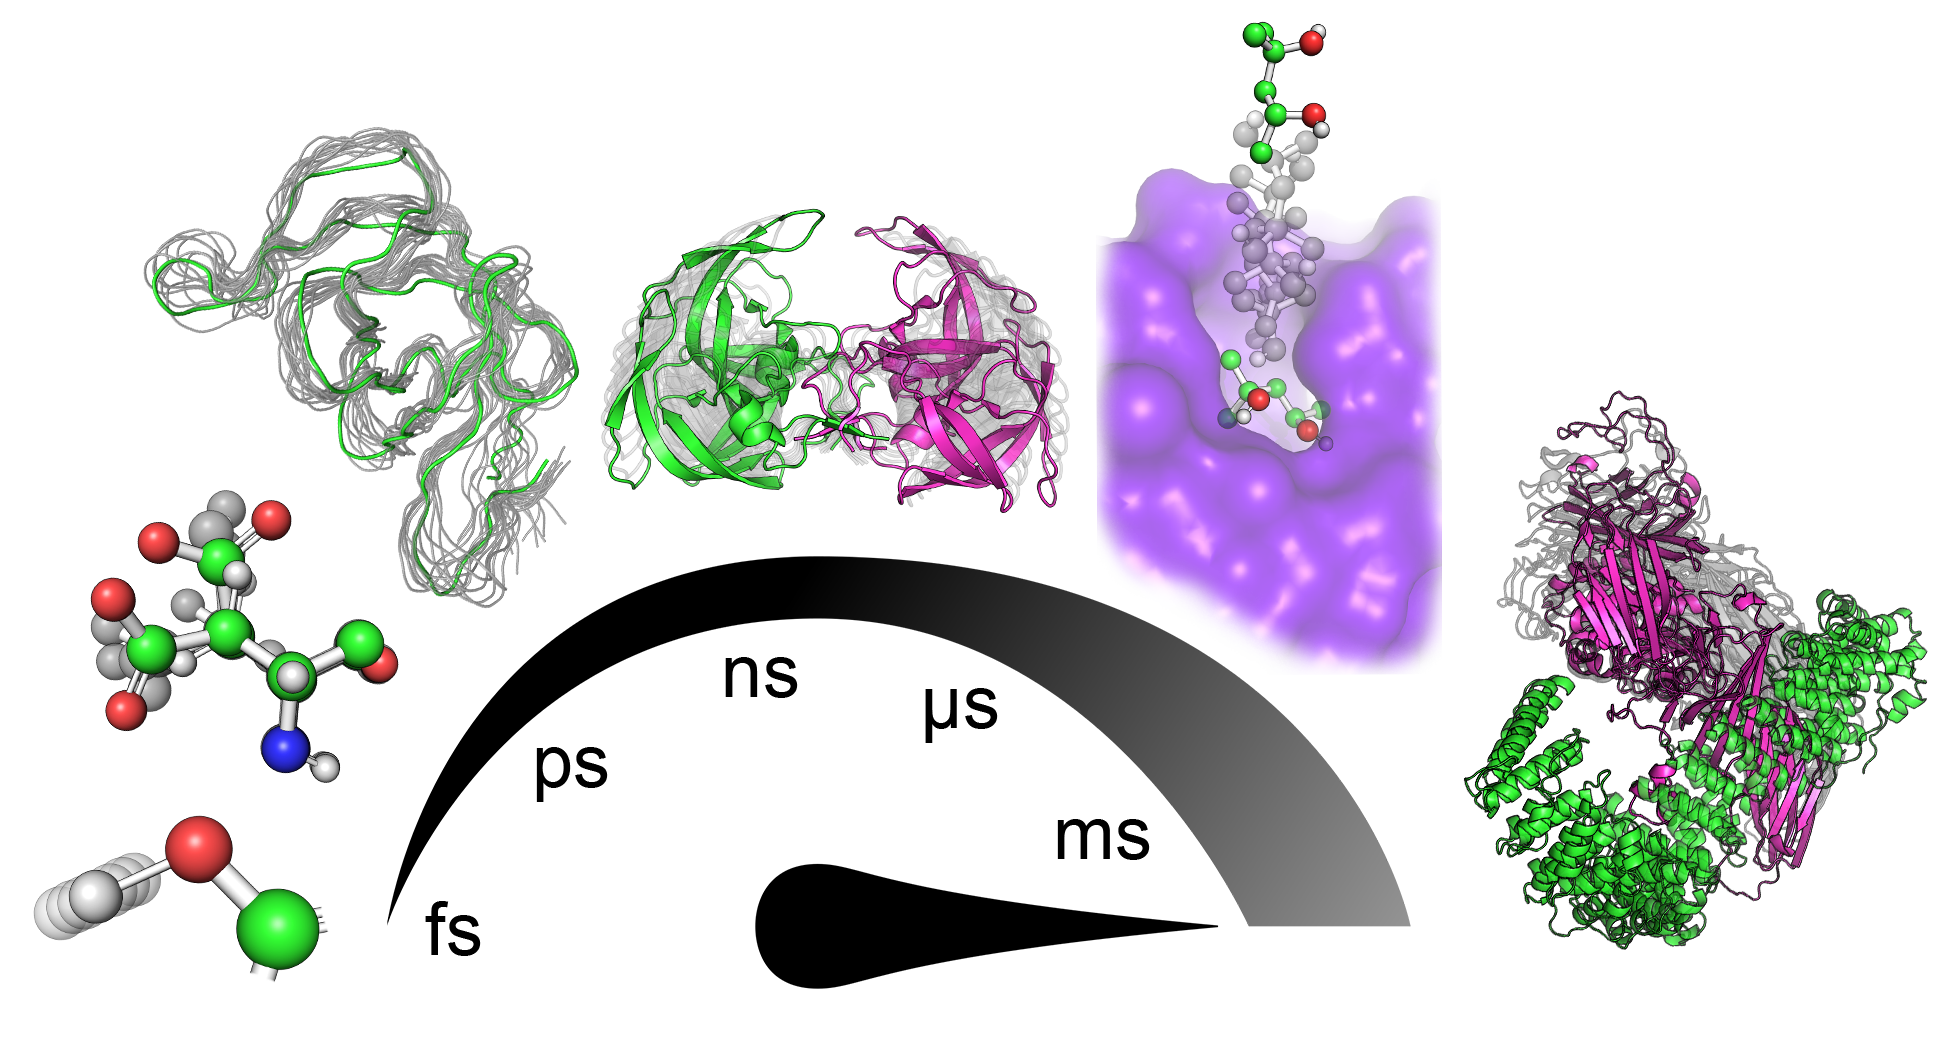
\includegraphics[height=0.65\textwidth,width=0.95\textwidth,viewport=0 0 470 290,clip]{Figures/Protein-structure.png}
%\caption{\textrm{ABINIT}的Si.in}
\label{Protein-structure-1}
\end{figure}
因此,力学常被冠以``动力学''的称呼
}

\frame
{
	\frametitle{\textrm{H}键与蛋白质分子的折叠}
\begin{figure}[h!]
\centering
\vspace{-5.5pt}
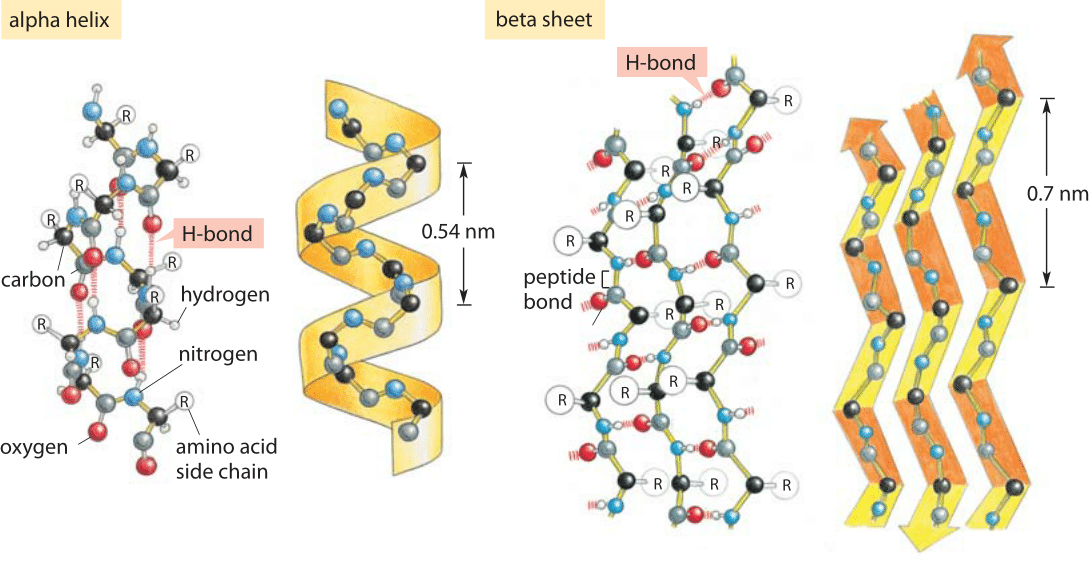
\includegraphics[height=0.57\textwidth,width=1.0\textwidth,viewport=0 0 1100 600,clip]{Figures/310-f1-AlphaBeta-1.png}
%\caption{\textrm{ABINIT}的Si.in}
\label{Protein-structure-2}
\end{figure}
}

%\frame
%{
%	\frametitle{分子动力学模拟:~蛋白质分子的折叠}
%\begin{figure}[h!]
%\centering
%\vspace{-5.5pt}
%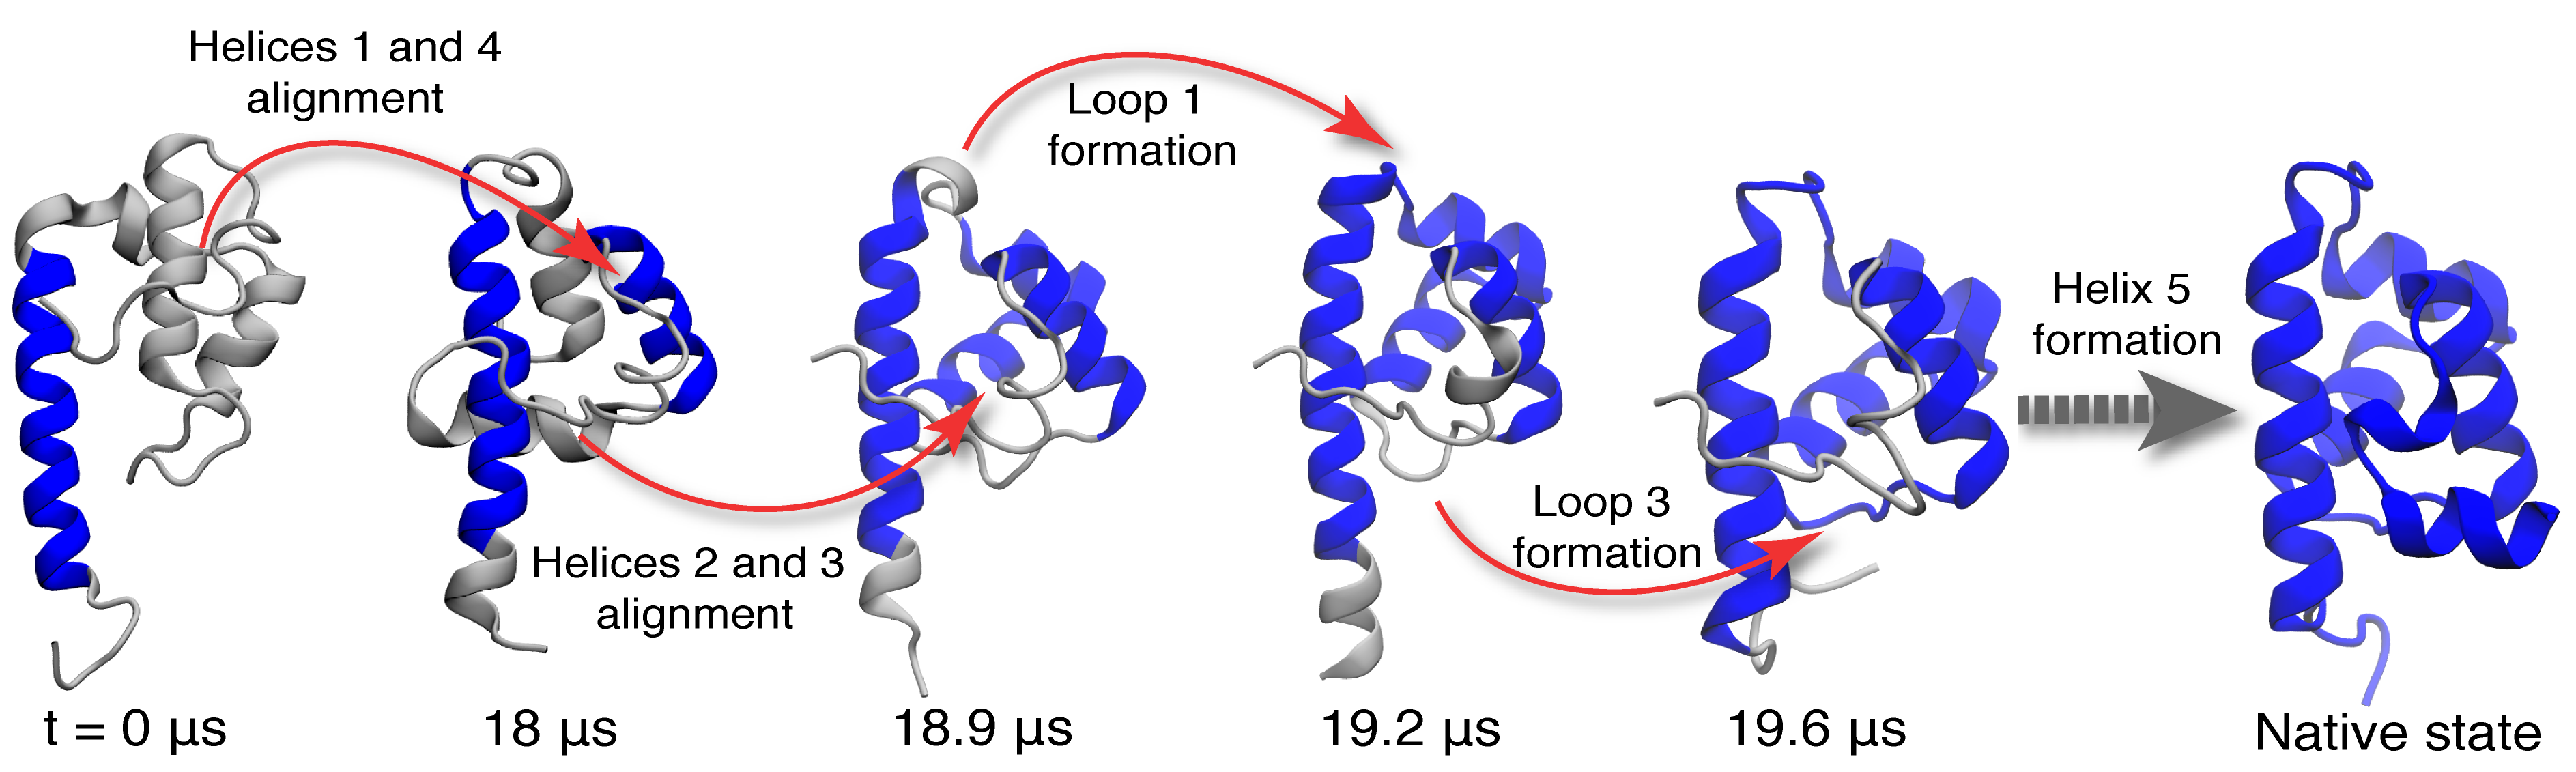
\includegraphics[height=0.30\textwidth,width=1.0\textwidth,viewport=0 0 1820 550,clip]{Figures/Protein-folding-2.png}
%%\caption{\textrm{ABINIT}的Si.in}
%\label{Protein-folding_1}
%\end{figure}
%}
%
\frame
{
	\frametitle{分子动力学模拟:~蛋白质分子的折叠}
\begin{figure}[h!]
\centering
\vspace{-13.5pt}
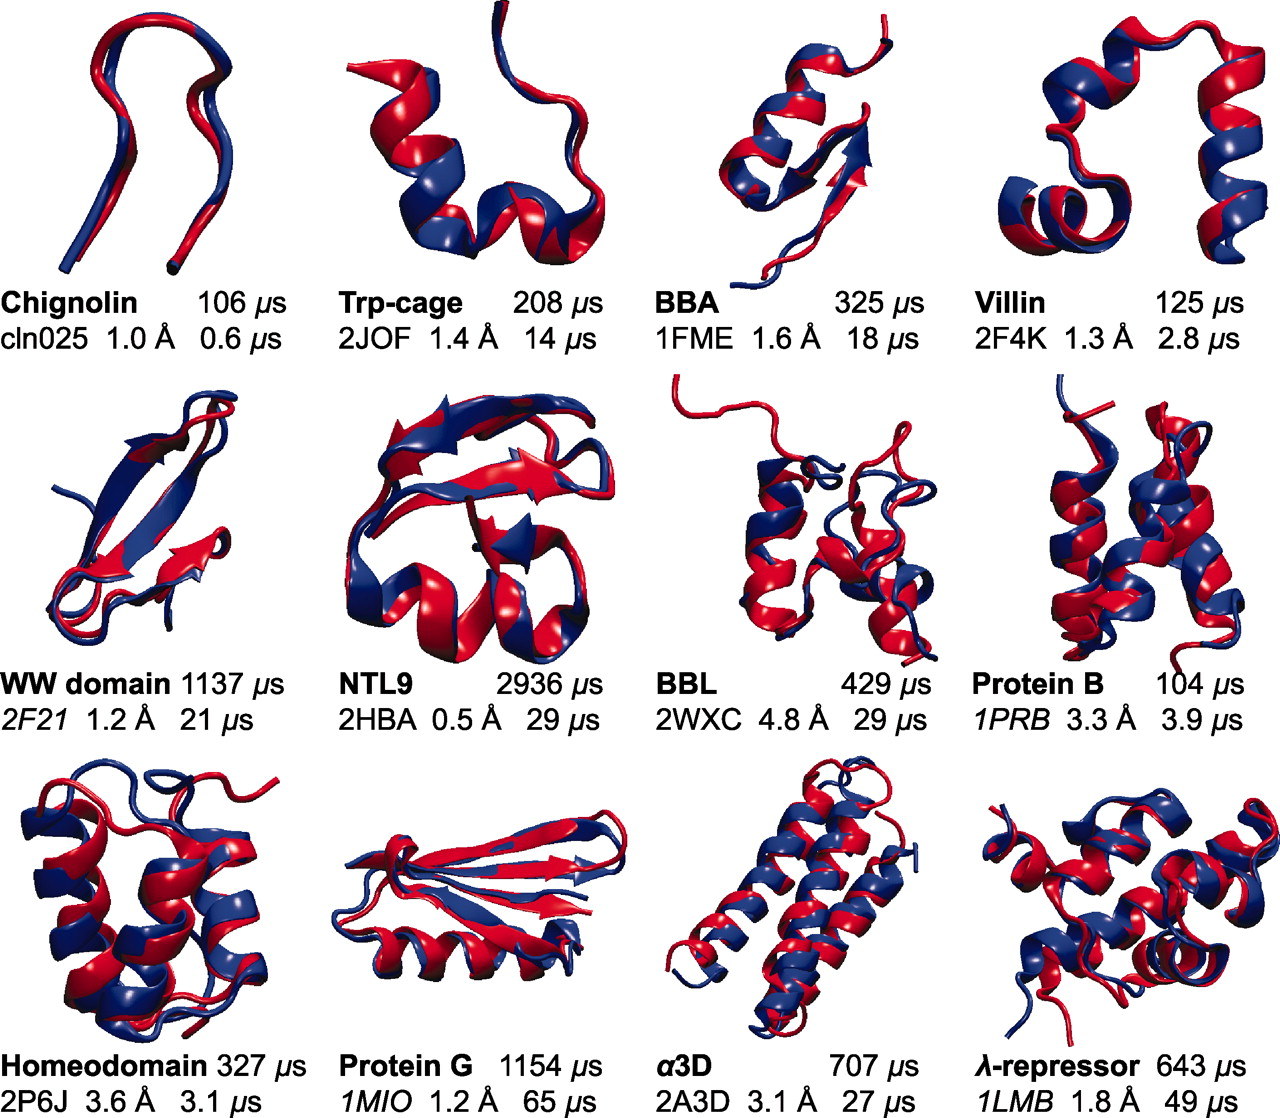
\includegraphics[height=0.75\textwidth,width=1.0\textwidth,viewport=0 0 1290 1130,clip]{Figures/Protein-folding.jpeg}
%\caption{\textrm{ABINIT}的Si.in}
\label{Protein-folding_2}
\end{figure}
}

\frame
{
	\frametitle{反应动力学:~酶与底物相互作用}
\begin{figure}[h!]
\centering
\vspace{-10.5pt}
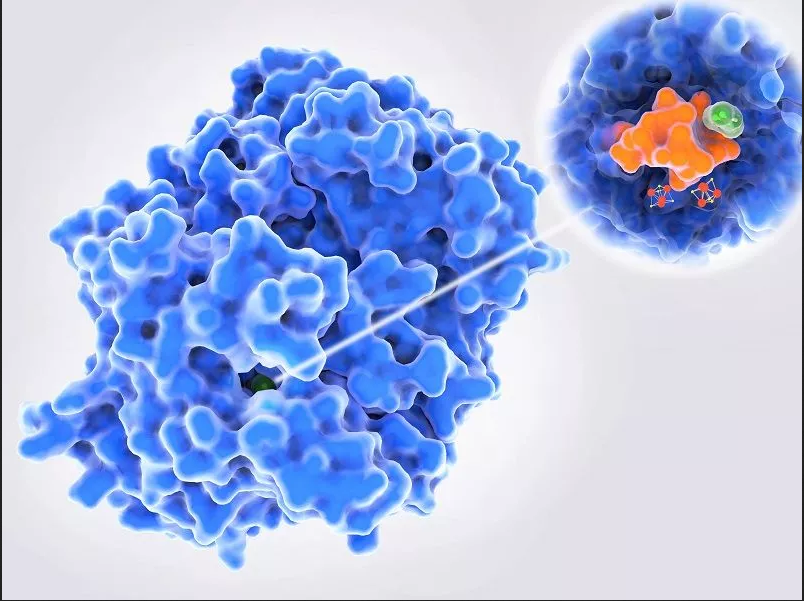
\includegraphics[height=0.30\textwidth,width=0.4\textwidth,viewport=0 0 880 600,clip]{Figures/Active_site_model.png}
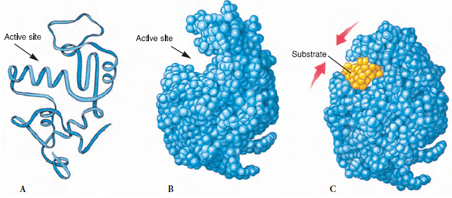
\includegraphics[height=0.37\textwidth,width=1.0\textwidth,viewport=0 0 460 200,clip]{Figures/enzyme-substrate-2.png}
%\caption{\textrm{ABINIT}的Si.in}
\label{enzyme-substrate}
\end{figure}
}

\subsection{分子间相互作用与化学键}
\frame
{
	\frametitle{分子间相互作用的本质}
\begin{figure}[h!]
\centering
\vspace{-10.5pt}
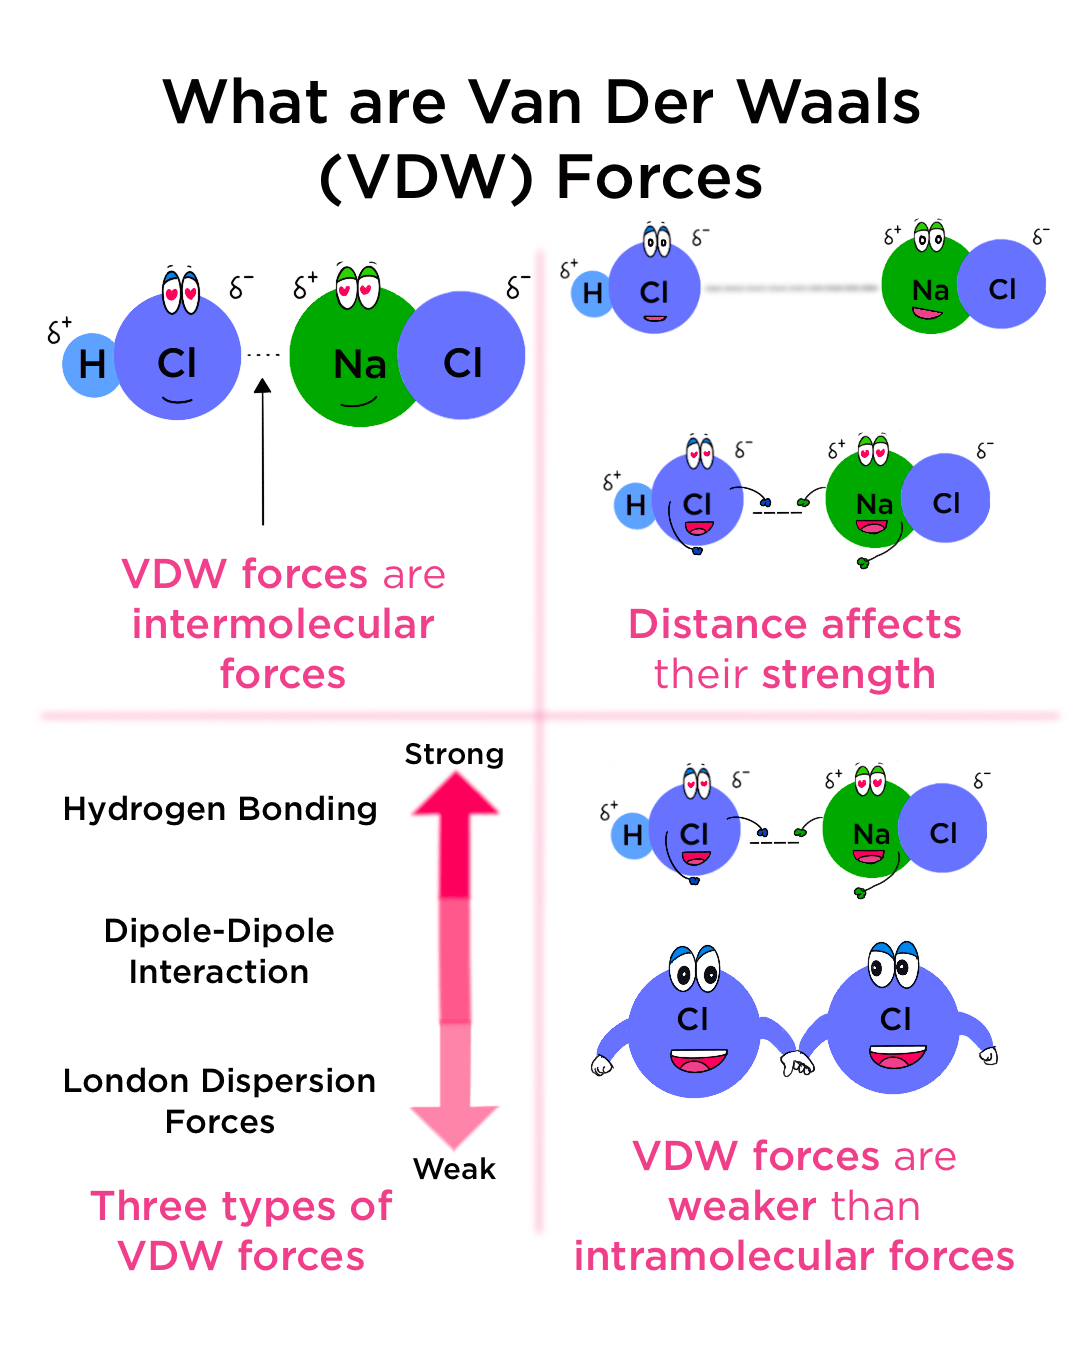
\includegraphics[height=1.65in ,width=1.55in,viewport=0 0 1150 1280,clip]{Figures/van_der_Waals-Force.png}\\
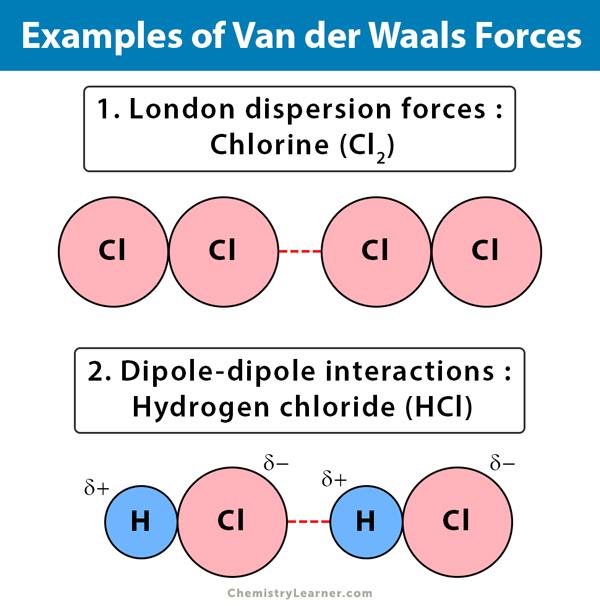
\includegraphics[height=1.30in,width=1.60in,viewport=0 25 600 530,clip]{Figures/Van-Der-Waals-Forces-Bond-Interactions-Examples.jpg}
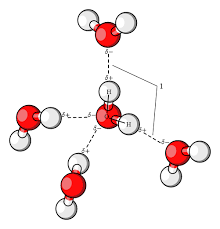
\includegraphics[height=1.30in,width=1.60in,viewport=0 0 280 230,clip]{Figures/water-H-bond.png}
%\caption{\textrm{ABINIT}的Si.in}
\label{van_der_Waalss}
\end{figure}
}

\subsection{从力场到化学键}
\frame
{
	\frametitle{原子:~原子核与电荷密度}
\begin{figure}[h!]
\centering
\vspace{3.5pt}
%\caption{\textrm{The wave-particle duality and Photoelectric effect}}
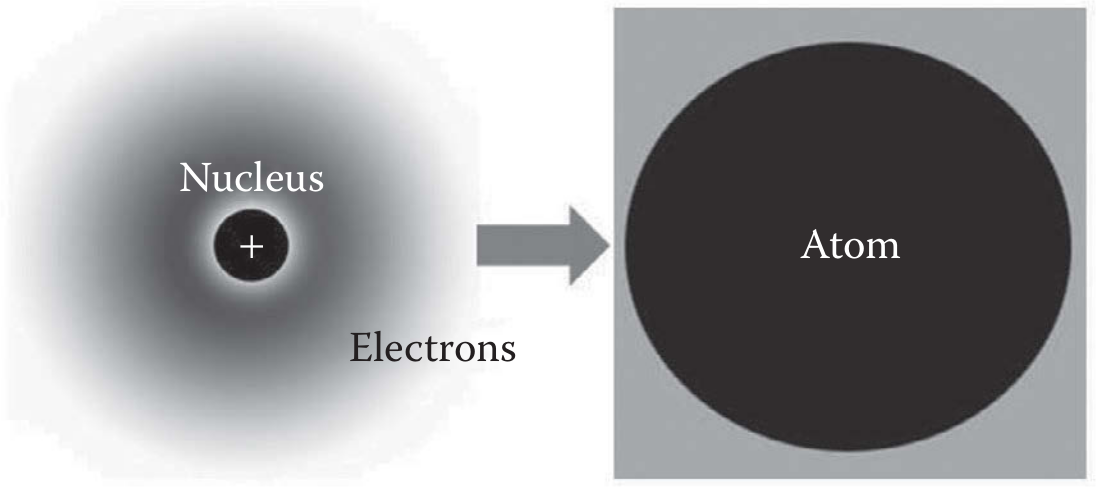
\includegraphics[height=1.90in,width=4.00in,viewport=0 0 1096 487,clip]{Figures/MD_atom_electron-nucleus.png}
\label{MO-Atom-Nuclear-electron}
\end{figure}
}

\frame
{
	\frametitle{原子间相互作用的经典描述:~力场}
\begin{figure}[h!]
\centering
\vspace{-10.5pt}
%\caption{\textrm{The wave-particle duality and Photoelectric effect}}
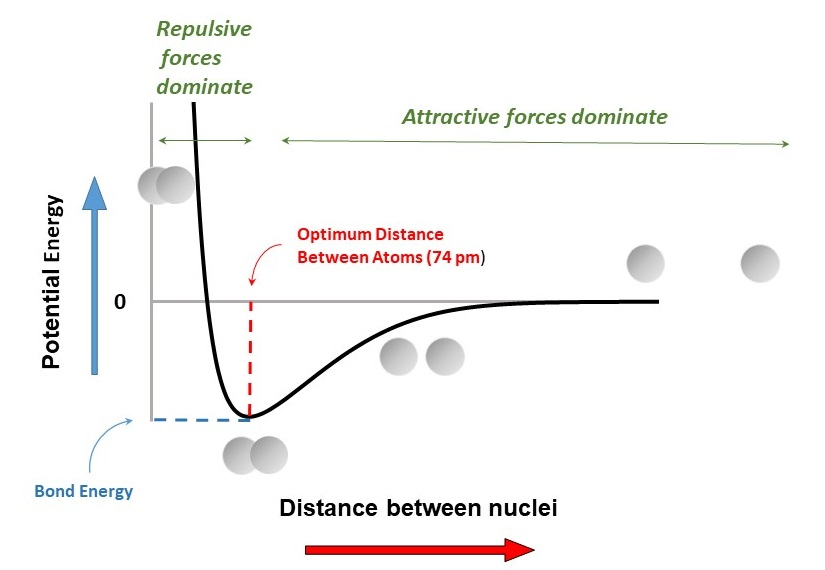
\includegraphics[height=1.45in,width=2.00in,viewport=0 0 600 430,clip]{Figures/H2-bonding.jpg}\\
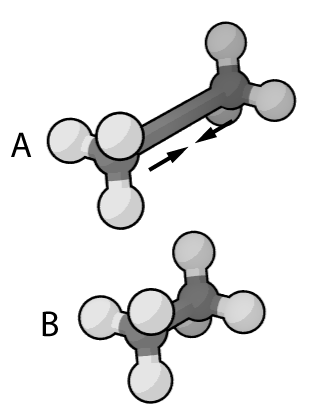
\includegraphics[height=1.45in,width=1.20in,viewport=0 0 323 420,clip]{Figures/Bond_stretching_energy.png}
\label{Bond_stretching-model}
\end{figure}
}

\frame
{
	\frametitle{原子间相互作用:~原子核/离子实与电荷密度}
\begin{figure}[h!]
\centering
\vspace{-10.5pt}
%\caption{\textrm{The wave-particle duality and Photoelectric effect}}
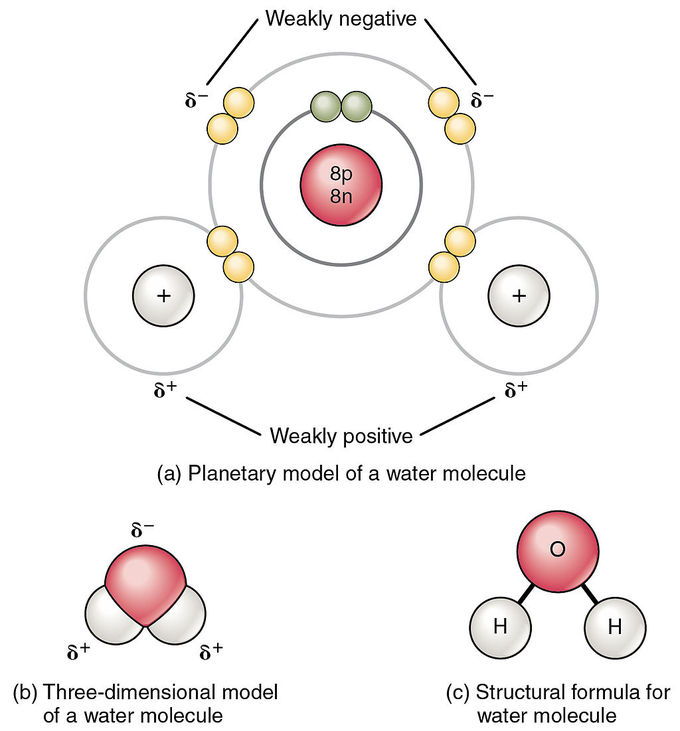
\includegraphics[height=1.70in,width=1.60in,viewport=0 0 170 180,clip]{Figures/Structure_of_water_molecule.jpg}\\
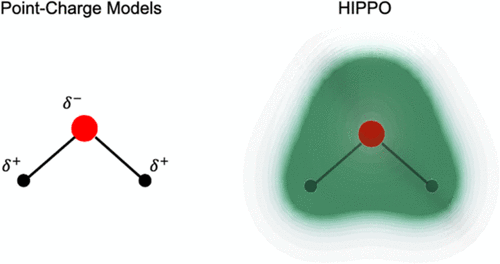
\includegraphics[height=1.20in,width=2.20in,viewport=0 0 480 280,clip]{Figures/H2O_bond.png}
\label{MO-Bond_model-H2O}
\end{figure}
}

\frame
{
	\frametitle{电荷密度与力场}
\begin{figure}[h!]
\centering
\vspace{-10.5pt}
%\caption{\textrm{The wave-particle duality and Photoelectric effect}}
\includegraphics[height=2.90in,width=3.2in,viewport=0 0 870 780,clip]{Figures/Molecular_electrostatic_potential_(MEP)-surface-and-fitting-point_charges-to-the-electrostatic_potential-of-N-(2_bromoethyl)_phthalimide.png}
\label{MO-potential_density}
\end{figure}
}

\frame
{
	\frametitle{力场的具象描述:~成键}
\begin{figure}[h!]
\centering
\label{MO-Bond_charge-density}
\vspace{-3.5pt}
%\caption{\textrm{The wave-particle duality and Photoelectric effect}}
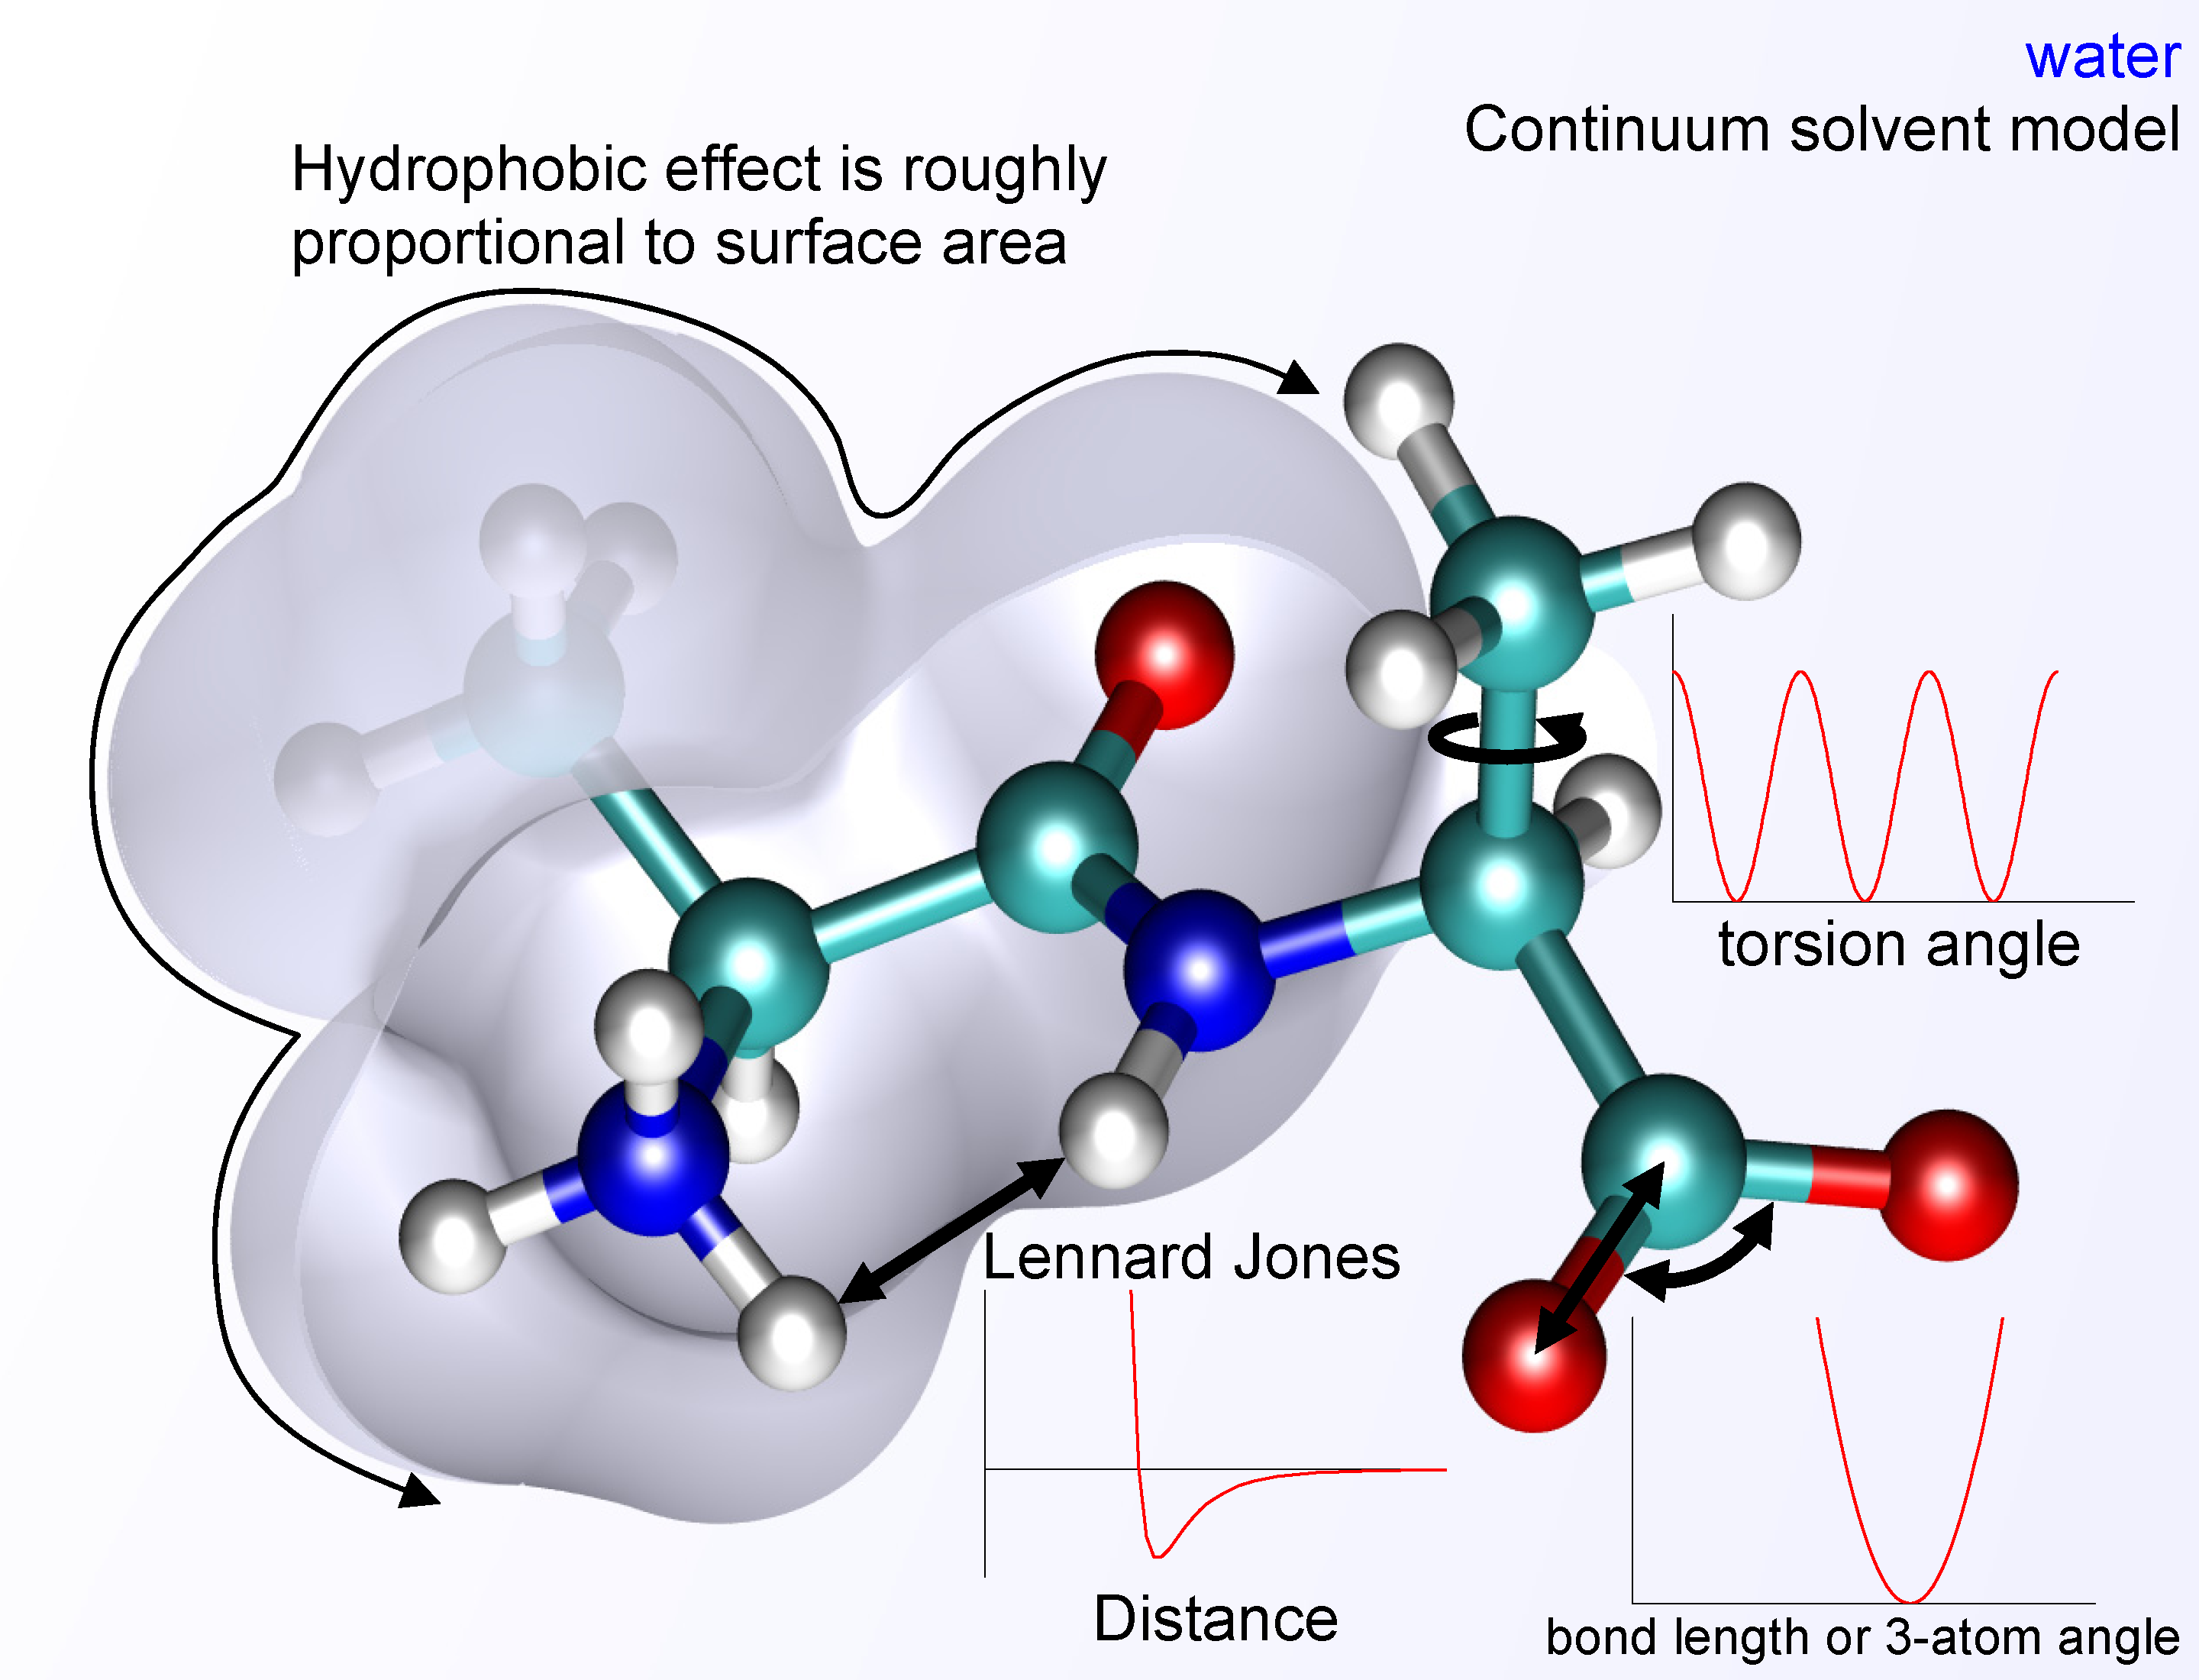
\includegraphics[height=2.70in,width=4.00in,viewport=0 0 355 260,clip]{Figures/Molecular_mechanics-potential_energy_function-with-continuum_solvent.png}
\end{figure}
}

\frame
{
	\frametitle{键与化学键}
\begin{figure}[h!]
\centering
\vspace{-10.5pt}
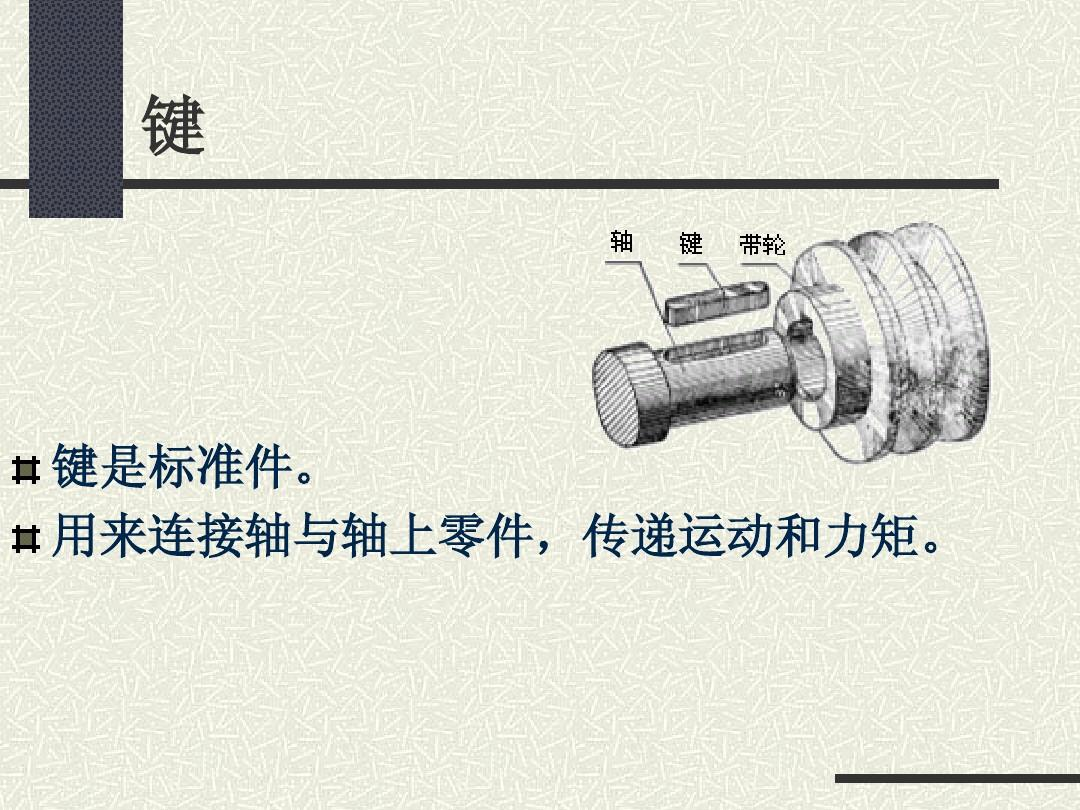
\includegraphics[height=1.00in ,width=2.60in,viewport=45 250 1000 590,clip]{Figures/Bond.jpeg}
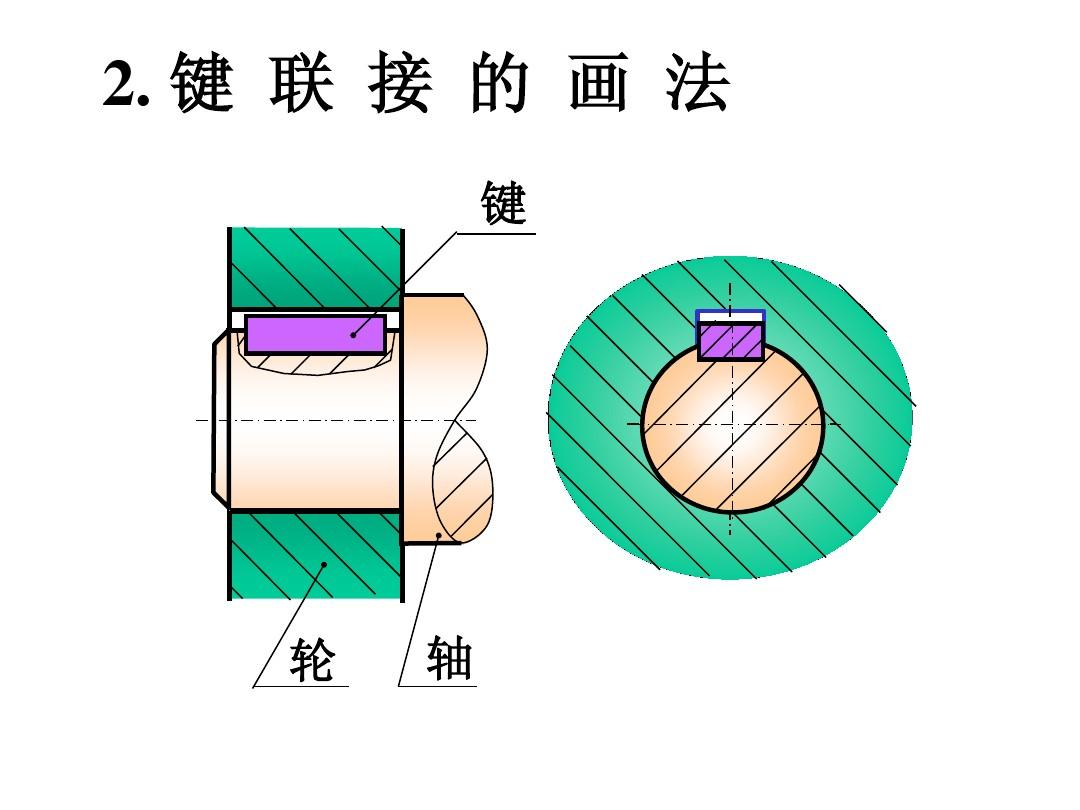
\includegraphics[height=1.00in,width=1.30in,viewport=180 110 915 650,clip]{Figures/Bond_2.jpeg}
%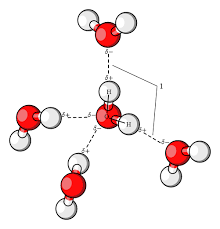
\includegraphics[height=1.30in,width=1.60in,viewport=0 0 280 230,clip]{Figures/water-H-bond.png}
%\caption{\textrm{ABINIT}的Si.in}
\label{Bond}
\end{figure}
\textcolor{blue}{化学键}(\textrm{chemical bond}):~物质内部相邻两个或多个原子(或离子)间强烈的相互作用力的统称
\begin{figure}[h!]
\centering
\vspace{-10.5pt}
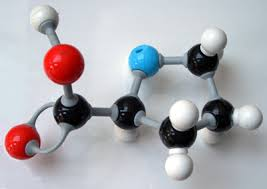
\includegraphics[height=1.30in,width=1.80in,viewport=0 0 315 210,clip]{Figures/Molecular-Chemical-bonding.jpeg}
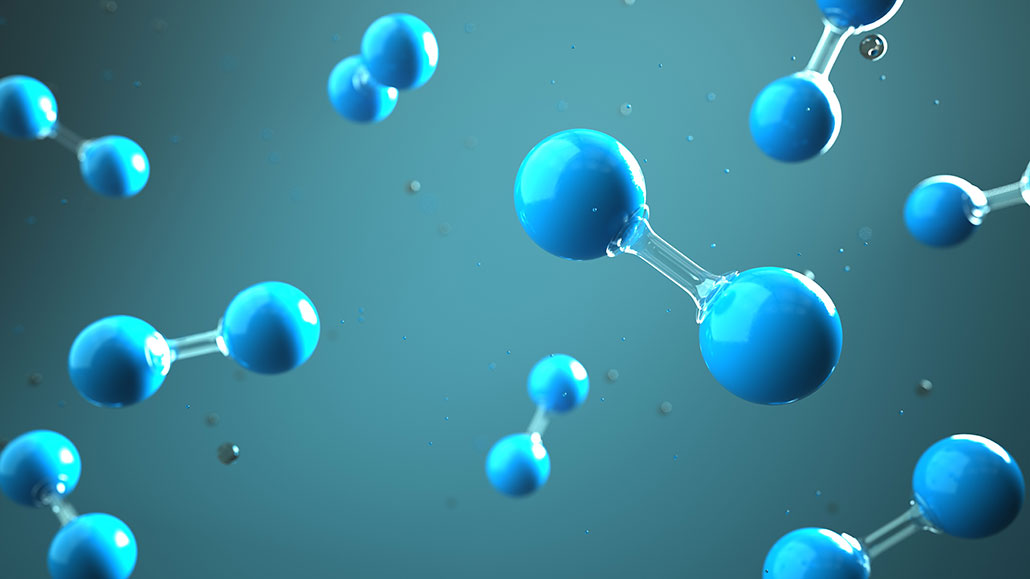
\includegraphics[height=1.30in,width=1.80in,viewport=0 0 1050 650,clip]{Figures/Chemical_Bonding_2.jpg}
%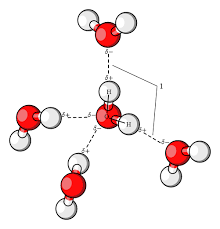
\includegraphics[height=1.30in,width=1.60in,viewport=0 0 280 230,clip]{Figures/water-H-bond.png}
%\caption{\textrm{ABINIT}的Si.in}
\label{Chemical_Bond-1}
\end{figure}
}

\frame
{
	\frametitle{化学键}
化学反应:~\textcolor{purple}{伴随旧的化学键的断裂和新的化学键的生成}
\begin{figure}[h!]
\centering
%\vspace{-5.5pt}
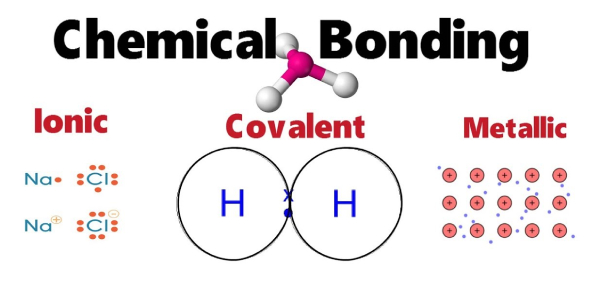
\includegraphics[height=0.50\textwidth,width=1.0\textwidth,viewport=0 0 580 280,clip]{Figures/Chemical_Bonding.jpg}
%\caption{\textrm{ABINIT}的Si.in}
\label{Chemical_Bond-2}
\end{figure}
{\centering\textcolor{magenta}{对化学键本质的认知:~时代呼唤量子力学}}
}

\section{量子力学简介}
\subsection{能量量子化}
%\frame
%{
%	\frametitle{经典物理学天空的“两朵乌云”\textrm{(Dark Clouds)}}
%\begin{figure}[h!]
%\vspace*{-0.18in}
%\centering
%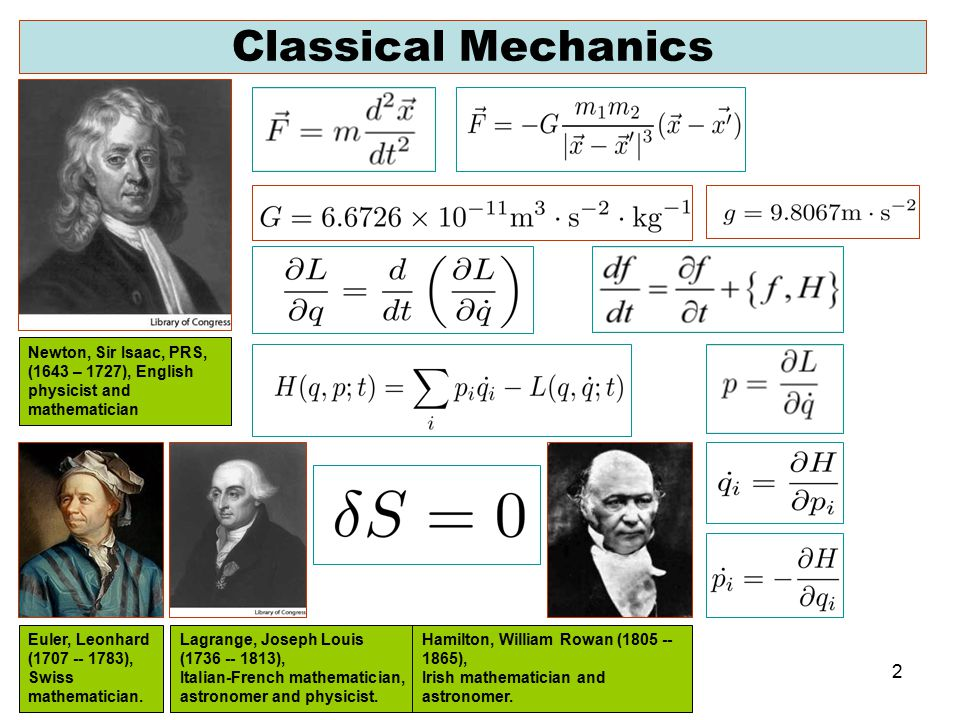
\includegraphics[height=2.65in,width=4.05in,viewport=0 0 715 495,clip]{Figures/Calssical_Mechanics.jpg}
%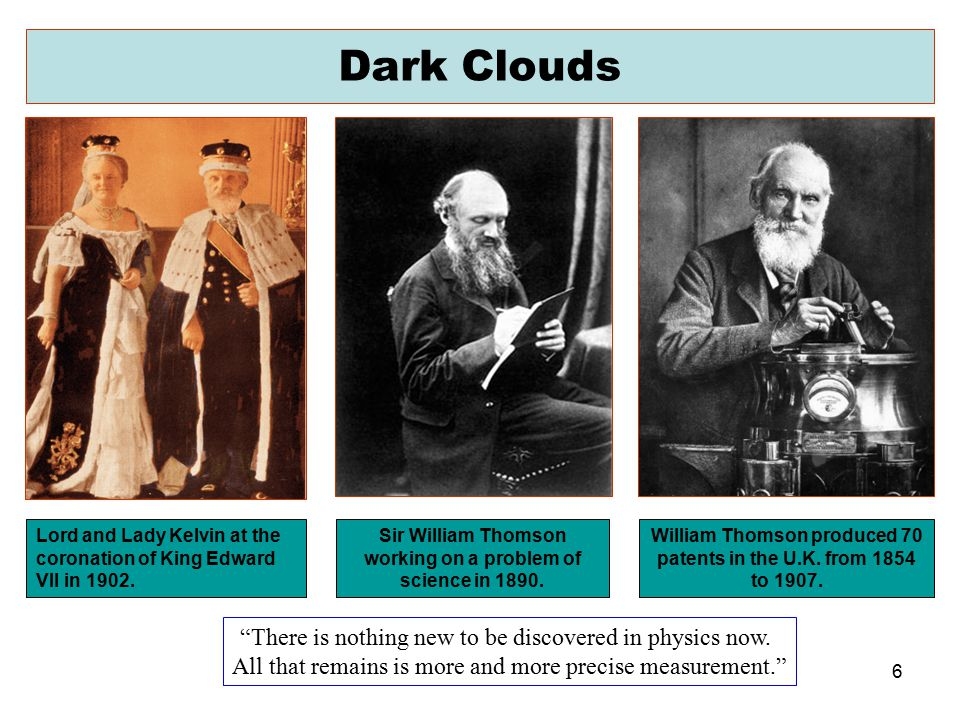
\includegraphics[height=2.50in,width=4.05in,viewport=0 20 735 470,clip]{Figures/Two-dark-cloud-in-physics-3.jpg}
%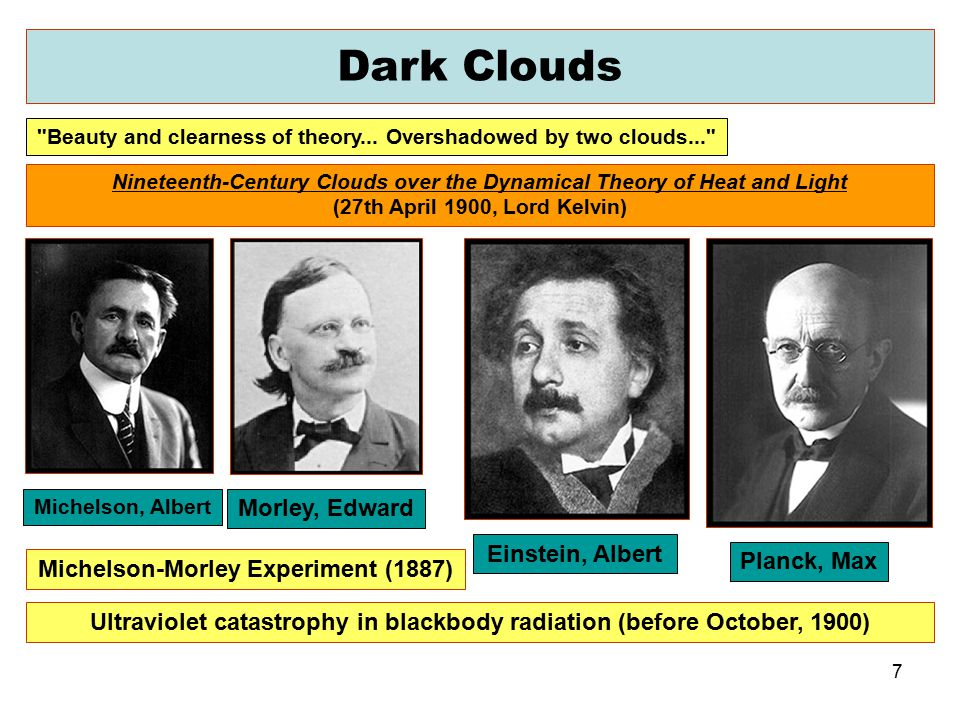
\includegraphics[height=2.40in,width=4.05in,viewport=0 50 735 470,clip]{Figures/Two-dark-cloud-in-physics-2.jpg}
%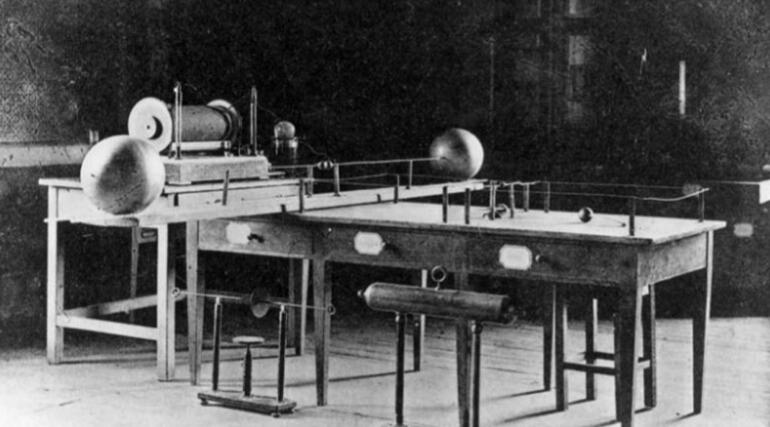
\includegraphics[height=2.40in,width=4.05in,viewport=0 0 580 325,clip]{Figures/Two-dark-cloud-in-physics-1.jpg}
%\label{two_Dark_Clouds}
%\end{figure}
%}

\frame
{
	\frametitle{黑体辐射与能量量子化}
	\textrm{1900}年,为了解释黑体辐射\textrm{(black-body radiation)}的能量密度与辐射频率的关系,\textrm{M.~Planck}引入\textcolor{red}{能量量子化}的假设,利用统计物理推导出与实验符合得非常好的黑体辐射\textrm{Planck~}公式:~
	\begin{displaymath}
		\rho_{\nu}\mathrm{d}{\nu}=\dfrac{8{\pi}h{\nu}^3}{C^3}\bigg(\dfrac1{\mathrm{e}^{h\nu/kT}-1}\bigg)\mathrm{d}\nu
	\end{displaymath}
\begin{figure}[h!]
\centering
\vspace{-10.5pt}
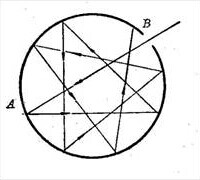
\includegraphics[height=1.45in,width=1.45in,viewport=0 0 136 136,clip]{Figures/Black_box.jpg}
\hskip 1pt
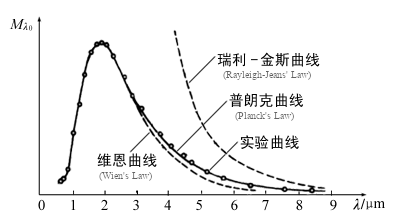
\includegraphics[height=1.32in,width=2.25in,viewport=0 0 390 215,clip]{Figures/Black_box_curve.png}
\caption{\textrm{The black-body radiation and the curve}}
\label{Black_box}
\end{figure}
}

\frame
{
	\frametitle{波粒二象性与光电效应}
\begin{figure}[h!]
\centering
\vspace{-15.5pt}
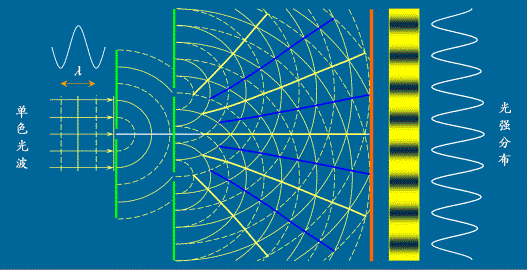
\includegraphics[height=1.35in,width=2.70in,viewport=0 0 536 280,clip]{Figures/wave-particle_duality.png}
\vskip 1pt
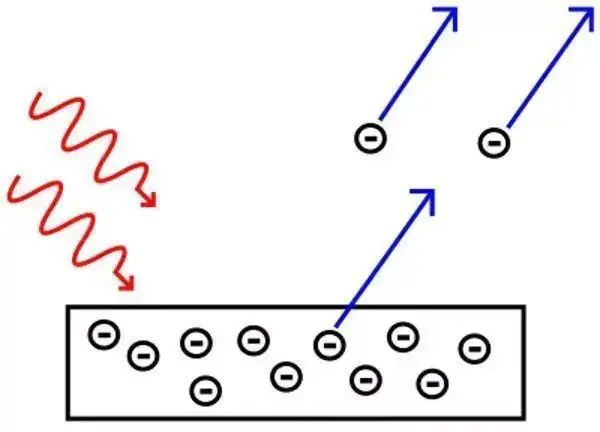
\includegraphics[height=1.32in,width=2.05in,viewport=0 0 620 455,clip]{Figures/Photoelectic_effect.png}
\caption{\textrm{The wave-particle duality and Photoelectric effect}}
\label{photo:wave_and_particle}
\end{figure}
}

\frame
{
	\frametitle{电子衍射、\textrm{Compton~effect}与\textrm{H}原子光谱}
\begin{figure}[h!]
\centering
\vspace{-15.5pt}
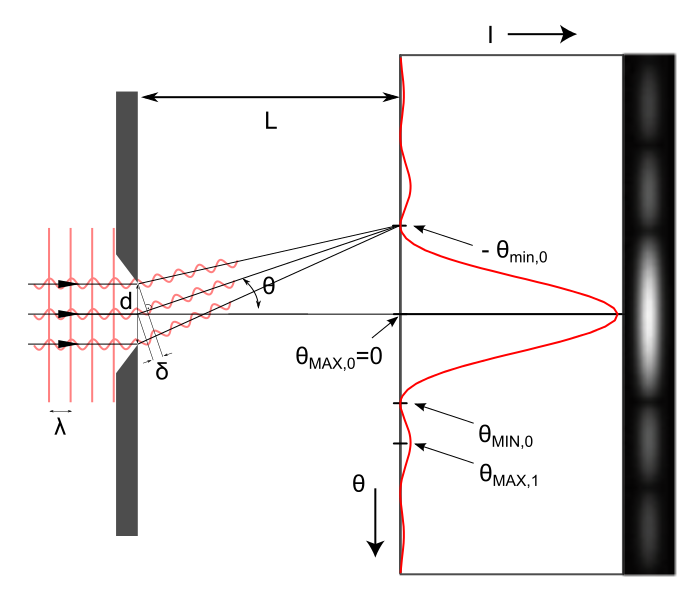
\includegraphics[height=1.35in,width=1.80in,viewport=0 0 680 600,clip]{Figures/Single_Slit_Diffraction.png}
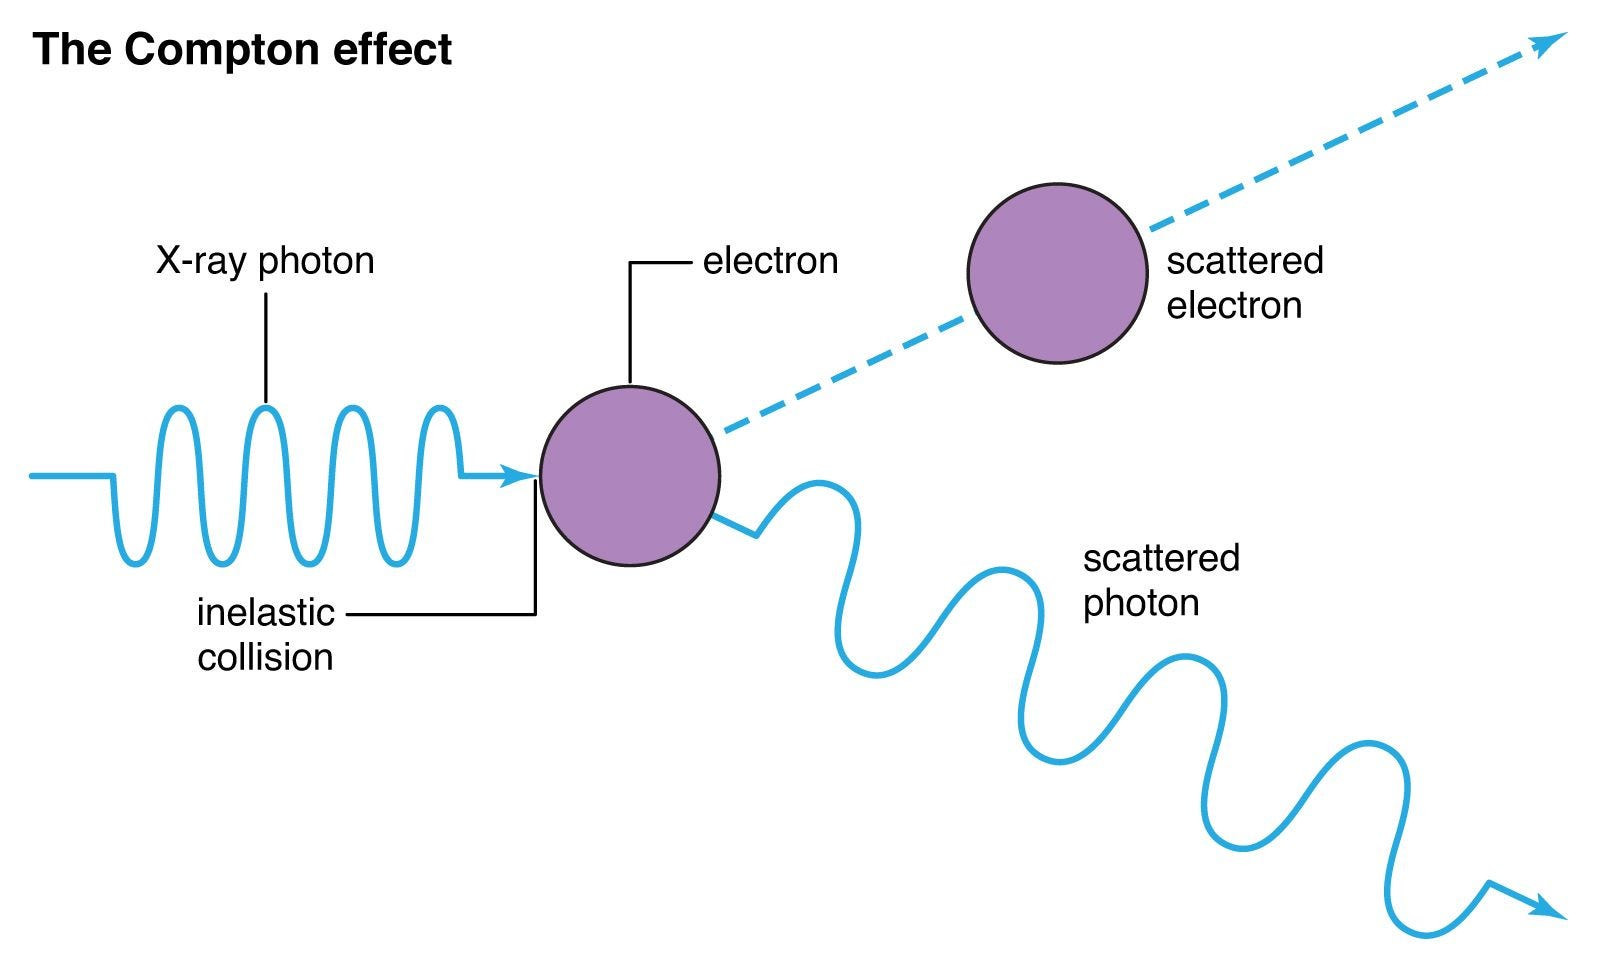
\includegraphics[height=1.20in,width=2.10in,viewport=0 0 1600 950,clip]{Figures/Compton_effect.jpg}\\
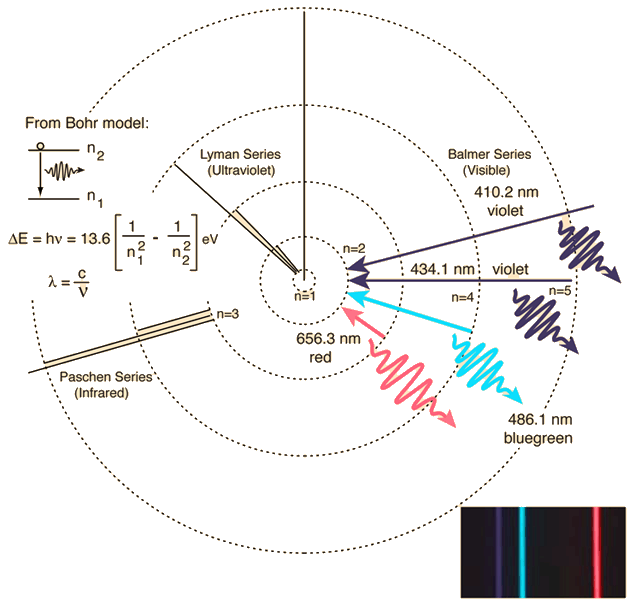
\includegraphics[height=1.65in,width=1.75in,viewport=0 0 620 600,clip]{Figures/Hydrogen_spectrum-3.png}
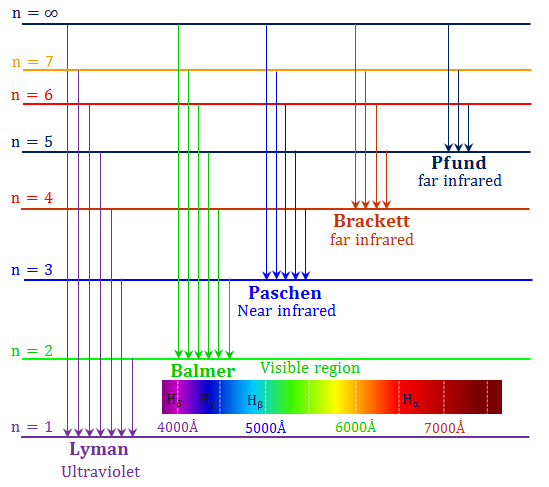
\includegraphics[height=1.55in,width=1.75in,viewport=0 0 500 380,clip]{Figures/Hydrogen_spectrum-2.png}
%\caption{\textrm{The wave-particle duality and Photoelectric effect}}
\label{electron:wave_and_particle}
\end{figure}
}

\subsection{\textrm{Schr\"odinger}方程与量子力学的建立}
\frame
{
	\frametitle{\textrm{De Broglie}物质波}
\begin{minipage}{0.53\textwidth}
\begin{figure}[h!]
\centering
\vspace{-15.5pt}
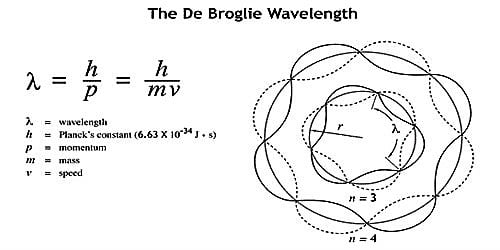
\includegraphics[height=1.3in,width=2.1in,viewport=0 0 500 280,clip]{Figures/De-Broglie-waves.jpg}
%\caption{\textrm{The wave-particle duality and Photoelectric effect}}
\label{Matter_wave}
\end{figure}
经典的观念:
\begin{itemize}
	\item \textcolor{red}{粒子}:~\textcolor{blue}{物质存在的形式}
	\item \textcolor{red}{波动}:~\textcolor{blue}{能量传递的形式}
\end{itemize}
\end{minipage}
\begin{minipage}{0.45\textwidth}
\begin{figure}[h!]
\centering
\vspace{-15.5pt}
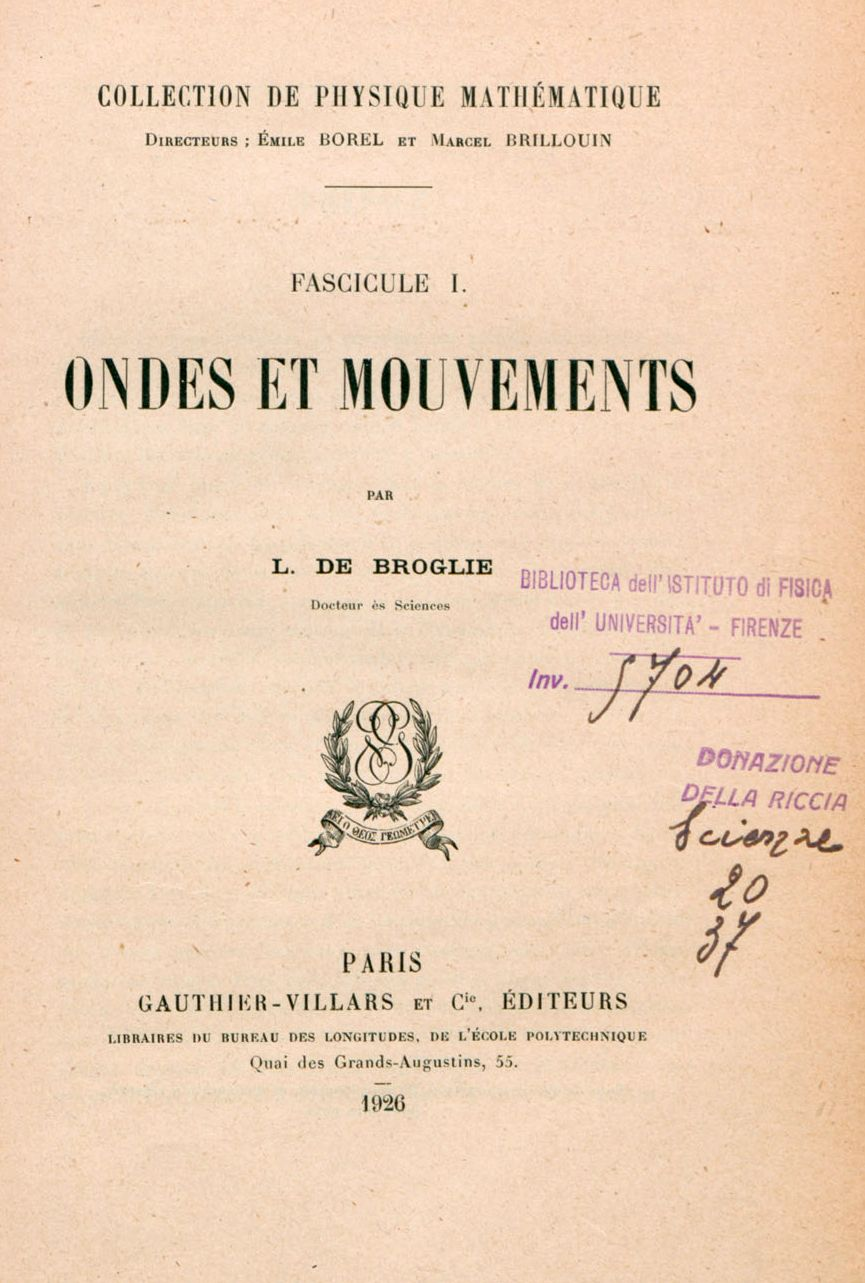
\includegraphics[height=2.80in,width=1.90in,viewport=0 0 430 650,clip]{Figures/De_Broglie-dissertation_Cover.jpg}
%\caption{\textrm{The wave-particle duality and Photoelectric effect}}
\label{De_Broglie-dissertation}
\end{figure}
\end{minipage}
}

\frame
{
	\frametitle{\textrm{驻波}}
\begin{figure}[h!]
\centering
\vspace{-15.5pt}
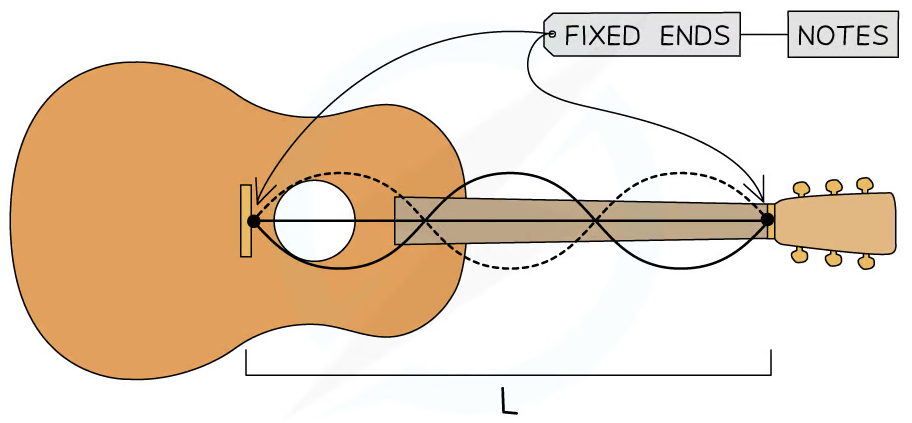
\includegraphics[height=0.40\textwidth,width=0.8\textwidth,viewport=0 0 900 450,clip]{Figures/Guitar-string.png}
\vskip 0.1pt
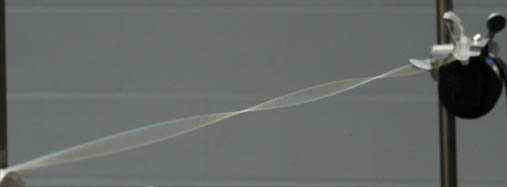
\includegraphics[height=0.35\textwidth,width=0.8\textwidth,viewport=0 0 122 48,clip]{Figures/string-standing-wave.jpg}
%\caption{\textrm{ABINIT}的Si.in}
\label{Standing_Wave_0}
\end{figure}
}

\frame
{
	\frametitle{驻波方程与势阱}
\begin{figure}[h!]
\centering
\vspace{-12.5pt}
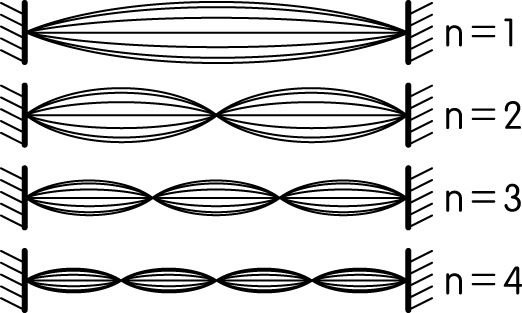
\includegraphics[height=0.32\textwidth,width=0.7\textwidth,viewport=0 0 125 75,clip]{Figures/Standing_wave.jpeg}
\vskip 2pt
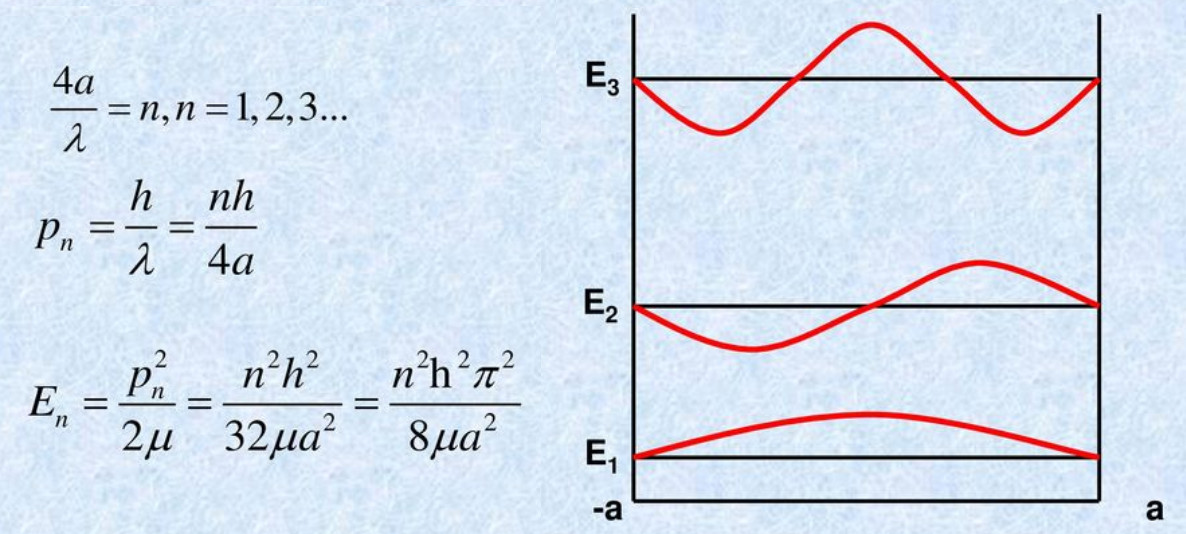
\includegraphics[height=0.40\textwidth,width=0.9\textwidth,viewport=0 0 1200 550,clip]{Figures/Standing_wave-energy.jpg}
%\caption{\textrm{ABINIT}的Si.in}
\label{Standing_Wave_1}
\end{figure}
}

\frame
{
	\frametitle{原子中电子的驻波方程}
\begin{figure}[h!]
	\vspace{-10.5pt}
\centering
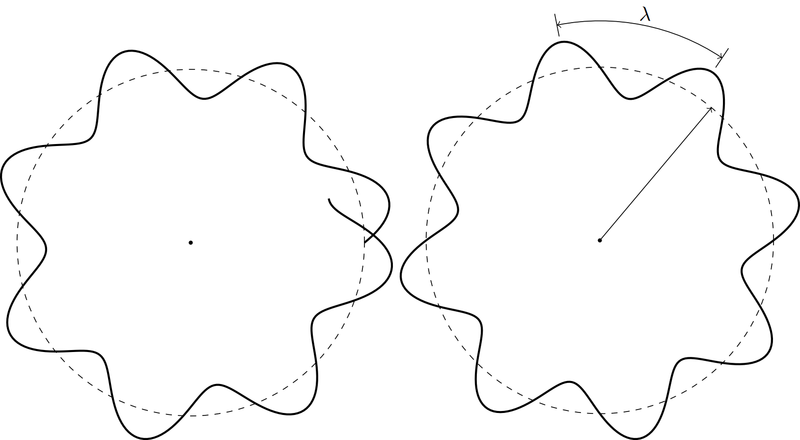
\includegraphics[height=0.38\textwidth,width=0.74\textwidth,viewport=0 0 840 440,clip]{Figures/Standing_wave-atom.png}
\vskip 2pt
\animategraphics[autoplay, loop, height=1.3in]{1}{Figures/Standing_wave_circle_}{1}{25}
\label{Atomic-electron_Standing_wave}
\end{figure}
}

\frame
{
	\frametitle{原子中的电子轨道和能量}
\begin{minipage}{0.43\textwidth}
\begin{figure}[h!]
%	\vspace{-14.8pt}
	\vspace{-4.8pt}
\centering
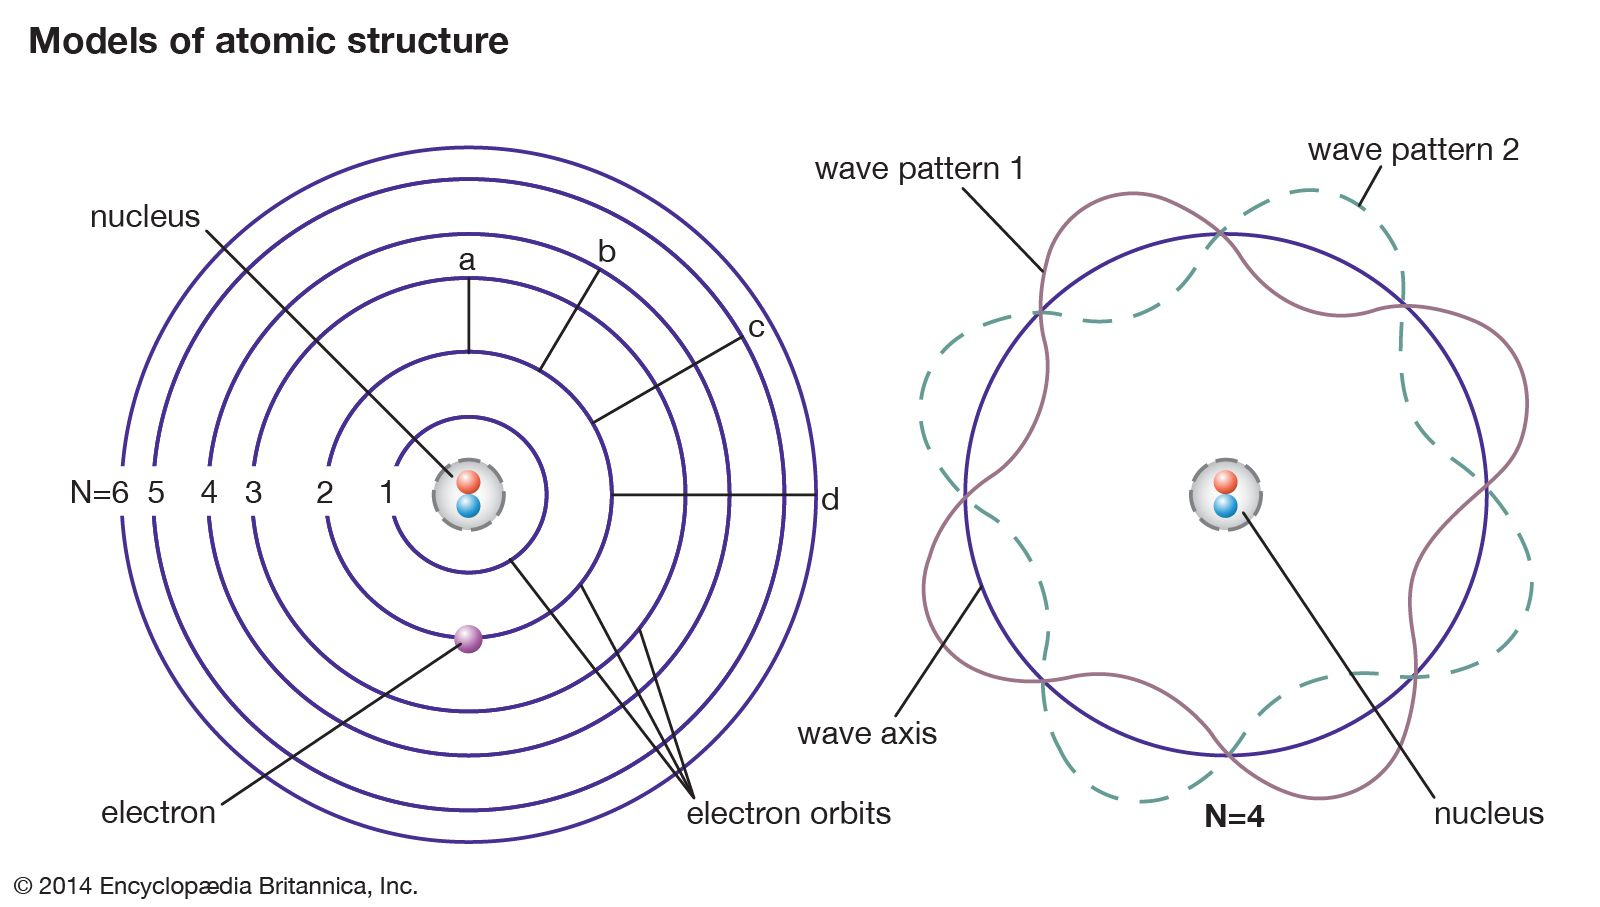
\includegraphics[height=0.57\textwidth,width=1.00\textwidth,viewport=0 50 1680 1000,clip]{Figures/electron-theory-Bohr-point-mass-energy-levels.jpg}
%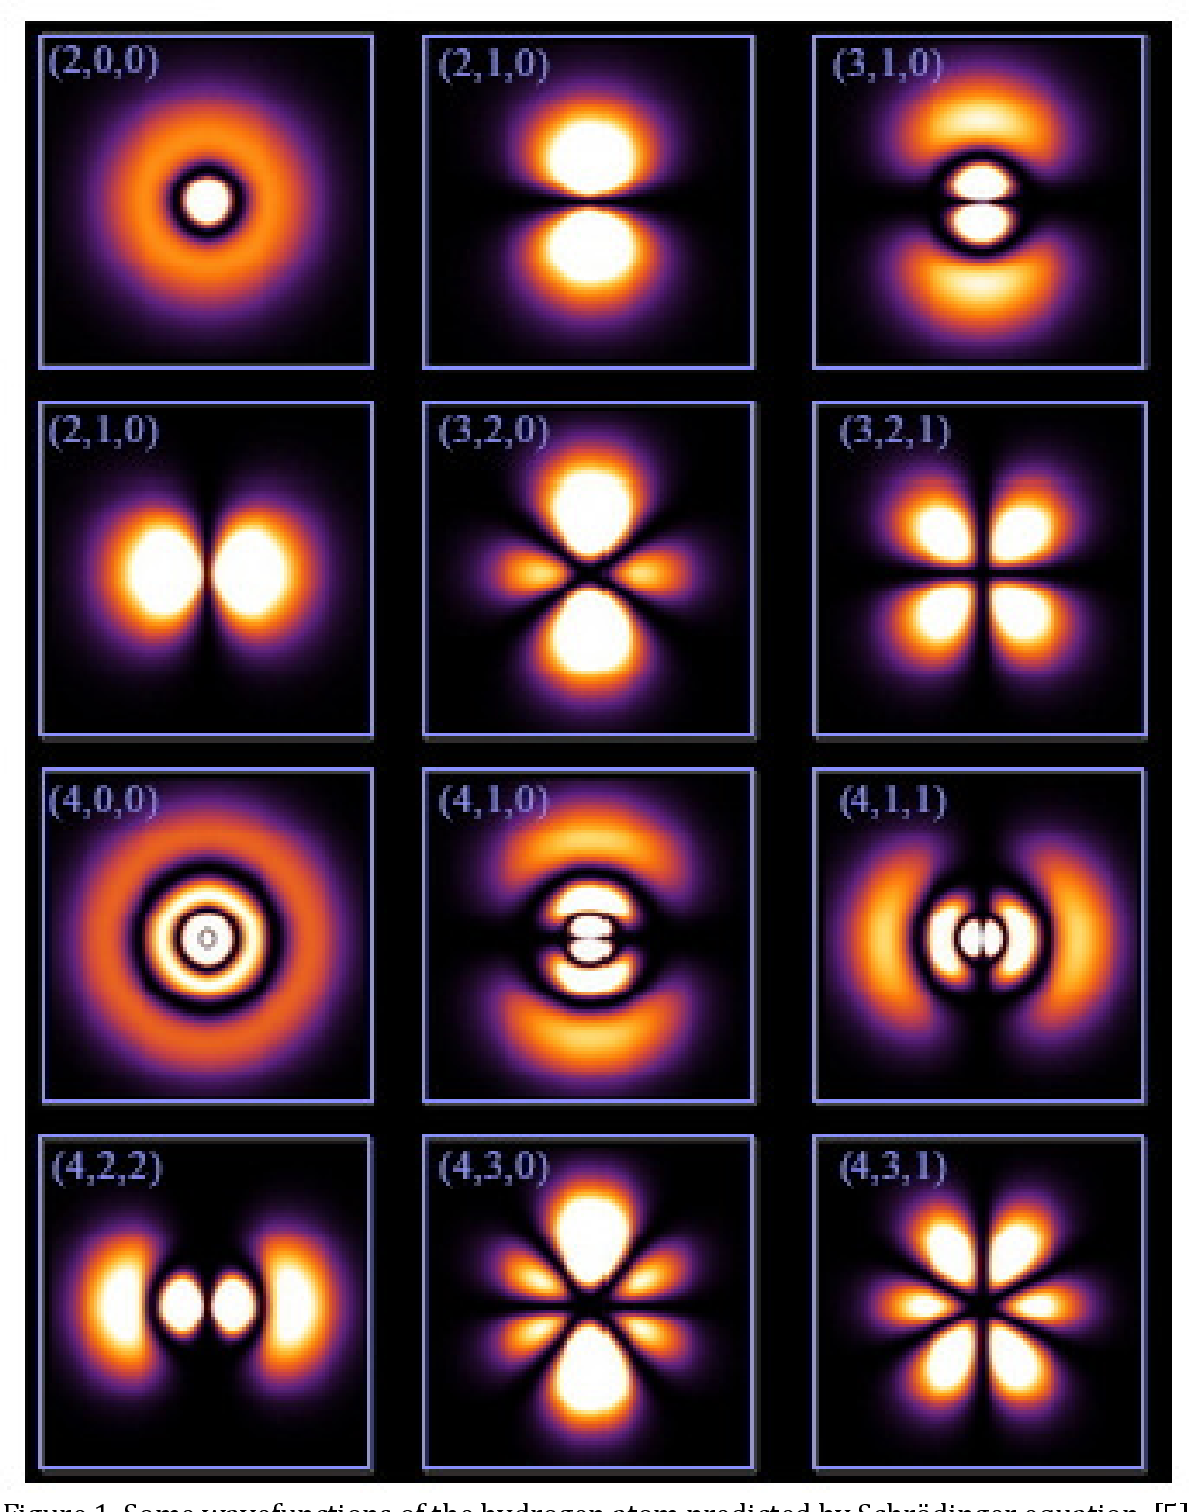
\includegraphics[height=1.23\textwidth,width=1.00\textwidth,viewport=0 10 1250 1500,clip]{Figures/wave_function.png}
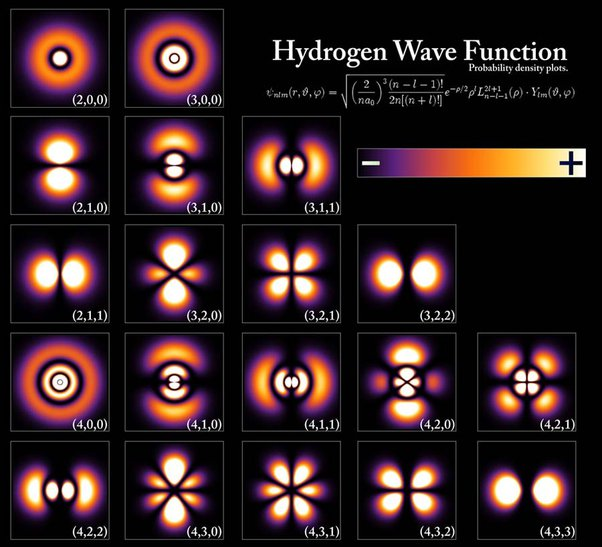
\includegraphics[height=0.95\textwidth,width=1.00\textwidth,viewport=0 0 630 650,clip]{Figures/wave_function-2.jpeg}
\label{Atomic-electron_wave}
\end{figure}
\end{minipage}
\begin{minipage}{0.55\textwidth}
\begin{figure}[h!]
	\vspace{-16.5pt}
\centering
\includegraphics[height=1.10\textwidth,width=1.00\textwidth,viewport=0 0 560 600,clip]{Figures/Electron_orbital-energy.png}
\label{Atomic-electron_wave-energy}
\end{figure}
\end{minipage}
}

\frame
{
	\frametitle{\textrm{Schr\"odinger}~方程}
\begin{minipage}{0.49\textwidth}
\begin{figure}[h!]
\centering
%
\vspace{-25.5pt}
\includegraphics[height=1.80in,width=2.00in,viewport=180 0 1380 1100,clip]{Figures/Schrodinger_article.png}
\includegraphics[height=1.20in,width=2.00in,viewport=0 0 600 350,clip]{Figures/Schrodinger_Equation.png}
\label{Schrodinger_Equation}
\end{figure}
\end{minipage}
\begin{minipage}{0.49\textwidth}
\begin{figure}[h!]
\centering
%
\vspace{-15.5pt}
\includegraphics[height=2.85in,width=2.00in,viewport=0 0 780 1100,clip]{Figures/Great_Equation.jpg}
\label{Great_Equation}
\end{figure}
\end{minipage}
}

\frame
{
	\frametitle{量子力学的奠基人}
\begin{figure}[h!]
\centering
%\vspace{-25.5pt}
%\hspace*{-15.5pt}
%\includegraphics[height=0.57\textwidth,width=1.1\textwidth,viewport=0 0 2150 1050,clip]{Figures/Solvay_Conference-5-fine.jpg}
\vspace{-14.5pt}
\hspace*{-15.5pt}
\includegraphics[height=0.50\textwidth,width=0.70\textwidth,viewport=150 105 850 710,clip]{Figures/Solvay_Conference-5.jpg}
\caption{\fontsize{7.5pt}{6.2pt}\selectfont{\textrm{The Fifth Solvay International Conference, Brussels, Belgium, Oct. 1927}}}
\label{Solvay Conference-5-fine}
\end{figure}
\vspace{-11.5pt}
\fontsize{4.1pt}{3.9pt}\selectfont{\textrm{\textcolor{blue}{前排左起}:~I.Langmuir(\textcolor{blue}{朗缪尔}) M.Planck(\textcolor{blue}{普朗克}) Marie Curie(\textcolor{blue}{居里夫人}) H.Lorentz(\textcolor{blue}{洛仑兹}) A.Einstein(\textcolor{blue}{爱因斯坦}) P.Langevin(\textcolor{blue}{朗之万}) Ch.E.Guye(\textcolor{blue}{古伊}) C.T.R.Wilson(\textcolor{blue}{威尔逊}) O.W.Richardson(\textcolor{blue}{理查森})\\
\textcolor{blue}{中排左起}:~P.Debye(\textcolor{blue}{德拜}) M.Knudsen(\textcolor{blue}{克努森}) W.L.Bragg(\textcolor{blue}{布拉格}) H.A.Kramers(\textcolor{blue}{克莱默}) P.A.M.Dirac(\textcolor{blue}{狄拉克}) A.H.Compton(\textcolor{blue}{康普顿}) L.de Broglie(\textcolor{blue}{德布罗意}) M.Born(\textcolor{blue}{玻恩}) N.Bohr(\textcolor{blue}{玻尔})\\
\textcolor{blue}{后排左起}:~A.Piccard(\textcolor{blue}{皮卡尔德}) E.Henriot(\textcolor{blue}{亨利厄特}) P.Ehrenfest(\textcolor{blue}{埃伦费斯特}) Ed.Herzen(\textcolor{blue}{赫尔岑}) Th.de Donder(\textcolor{blue}{德唐德}) E.Schr\"odinger(\textcolor{blue}{薛定谔}) E.Verschaffelt(\textcolor{blue}{费尔夏费尔特}) W.Pauli(\textcolor{blue}{泡利}) W.Heisenberg(\textcolor{blue}{海森堡}) R.H.Fowler(\textcolor{blue}{富勒}) L.Brillouin(\textcolor{blue}{布里渊})}}
}
%------------------------------------------------------------------------Reference----------------------------------------------------------------------------------------------
\frame
{
	\frametitle{态叠加原理:~\textrm{Schr\"odinger's cat}}
\begin{figure}[h!]
\centering
\vspace{-10.5pt}
\includegraphics[height=0.70\textwidth,width=0.48\textwidth,viewport=0 0 550 750,clip]{Figures/Schrodinger-cat.jpg}
\includegraphics[height=0.70\textwidth,width=0.50\textwidth,viewport=0 0 720 930,clip]{Figures/Schrodinger_book.jpg}
%\caption{\textrm{ABINIT}的Si.in}
\label{Schrodinger-cat}
\end{figure}
}

%\frame
%{
%	\frametitle{因果倒置:~\textrm{Delayed Choice Experiment}}
%\begin{figure}[h!]
%\centering
%\vspace{-10.5pt}
%\includegraphics[height=0.55\textwidth,width=1.0\textwidth,viewport=0 0 690 370,clip]{Figures/Schematic-diagram-of-delayed_choice-experiment.png}
%\caption{\fontsize{5.2pt}{3.9pt}\selectfont{\textrm{Schematic diagram of Wheeler's delayed choice experiment with A Mach-Zehnder Interferometer.}}}
%\label{Delayed_Choice-Experiment}
%\end{figure}
%}
%
\frame
{
	\frametitle{量子力学量力学}
\begin{figure}[h!]
\centering
\vspace{-13.5pt}
\includegraphics[height=0.75\textwidth,width=0.55\textwidth,viewport=0 0 500 650,clip]{Figures/Quote-Niels_Bohr-on-Quantum_mechanics.png}
\caption{\fontsize{5.2pt}{3.9pt}\selectfont{\textrm{A quote of Niels Bohr on Quantum mechanics.}}}
\label{Quote-Niels_Bohr}
\end{figure}
}

\frame
{
	\frametitle{几何原本:~公理体系的源头}
\begin{figure}[h!]
\centering
\vspace{-13pt}
\includegraphics[height=0.38\textwidth,width=0.65\textwidth,viewport=0 0 680 500,clip]{Figures/Element_Geometry_1.jpg}\\
\vspace{1pt}
\includegraphics[height=0.36\textwidth,width=0.65\textwidth,viewport=0 0 810 500,clip]{Figures/Element_Geometry_2.jpg}
%\caption{\textrm{ABINIT}的Si.in}
\label{Element_Geometru}
\end{figure}
}

\begin{frame}
	\frametitle{数的信仰}
\begin{figure}[h!]
\centering
\vspace{-15.5pt}
\includegraphics[height=1.30in,width=2.60in,viewport=0 0 600 290,clip]{Figures/pythagorean_numerology.png}
\includegraphics[height=1.20in,width=2.60in,viewport=0 0 850 400,clip]{Figures/quote_pythagoras.jpg}
\caption{\tiny 万物皆数\textrm{(All is number)}信仰}
\label{Pythagoras_numerology}
\end{figure}
\end{frame}

\begin{frame}
	\frametitle{无理数的挑战}
	\begin{itemize}
		\item \textcolor{red}{有理数}:~\textrm{rational number} ~~~ {\fontsize{7.5pt}{6.0pt}\selectfont{\textcolor{magenta}{\textrm{rate}} $\Longrightarrow$ \textrm{ration} $\longrightarrow$ \textcolor{violet}{\textrm{rational}}}}
		\item \textcolor{blue}{无理数}:~\textrm{irrational number}
	\end{itemize}
\begin{figure}[h!]
\centering
\vspace{-10.5pt}
\includegraphics[height=1.80in,width=1.80in,viewport=0 0 110 110,clip]{Figures/Pi_sqrt2.jpeg}
\includegraphics[height=1.80in,width=1.80in,viewport=0 0 317 316,clip]{Figures/coordinate-plane.png}
\caption{\tiny \textrm{$\pi$、$\sqrt 2$、$\sqrt 3$ from a circle and a coordinate plane.}}
\label{Pi_sqrt2}
\end{figure}
\end{frame}

\begin{frame}
	\frametitle{复数的物理意义}
	\begin{displaymath}
		\textcolor{blue}{z}=a+b\textcolor{red}{\mathbf{i}}
	\end{displaymath}
\begin{figure}[h!]
\centering
\vspace{-5.5pt}
\includegraphics[height=1.90in,width=4.00in,viewport=0 0 1052 566,clip]{Figures/RLC_series_circuit.png}
\caption{\tiny \textrm{The imaginary in RLC series circuit.}}
\label{complex_imaginary}
\end{figure}
\end{frame}

\frame
{
	\frametitle{\textcolor{red}{公理体系}:~现代科学的逻辑起点}
\begin{figure}[h!]
\centering
\vspace{-10.5pt}
\includegraphics[height=0.68\textwidth,width=1.0\textwidth,viewport=0 0 770 500,clip]{Figures/Philp_Nature_Mach-2.png}
%\caption{\textrm{ABINIT}的Si.in}
\label{Philp_Nature}
\end{figure}
}

\frame
{
	\frametitle{量子力学基本假设(\textcolor{red}{公理体系})}
	\begin{itemize}
		\item 波函数假设\\
			\textcolor{blue}{微观体系的运动状态可由波函数$\Psi$完全描述,波函数包含体系的所有性质}\\
			波函数$\Psi$一般要求满足\textcolor{red}{连续}、\textcolor{red}{有限}和\textcolor{red}{单值}三个条件
		\item 全同粒子假设\\
			\textcolor{blue}{全同粒子组成的体系中,两个全同粒子相互调换不改变体系的状态}\\ 
			全同粒子是指\textcolor{red}{内禀性质完全相同的一类微观粒子}:\\例如,所有的电子是全同粒子 
		\item 态叠加原理\\
			如果$\Psi_1$是体系的一个本征态,对应的本征值为$A_1$,$\Psi_2$也是体系的一个本征态,对应的本征值为$A_2$,则\textcolor{blue}{$$\Psi=C_1\Psi_1+C_2\Psi_2$$}\textcolor{red}{也是体系一个可能的存在状态}
	\end{itemize}
}

\frame
{
	\frametitle{叠加态的数学表示:~矩阵}
\begin{figure}[h!]
\centering
\vspace{-1.5pt}
\hspace*{-0.12in}
\includegraphics[height=0.48\textwidth,width=1.05\textwidth]{Figures/Matrix_Rotation.png}
%\caption{\textrm{ABINIT}的Si.in}
\label{Matrix-Rotation}
\end{figure}
}

%\frame
\frame
{
	\frametitle{量子力学基本假设(续)}
	\begin{itemize}
		\item 力学量算符假设\\
			\textcolor{blue}{经典力学中的物理量对应到量子力学中,要用线性\textrm{Hermite~}算符表示}(\textcolor{red}{\textrm{Hermite~}算符的本征函数构成完备空间})\\
			如动量算符 
			$$\hat{\mathbf{p}}=-\mathrm{i}\hbar\nabla$$
			位置算符$$\hat{\mathbf r}=r$$
			力学量算符之间有确定的对易关系(\textcolor{brown}{量子条件})
			$$[\hat{\mathbf F},\hat{\mathbf G}]=\hat{\mathbf F}\hat{\mathbf G}-\hat{\mathbf G}\hat{\mathbf F}$$ 
			
		\item 微观体系的运动状态\textcolor{blue}{波函数随时间变化的规律}:\\\textcolor{red}{遵从\textrm{Schr\"odinger}方程}
			$$\mathrm{i}\hbar\dfrac{\mathrm{d}}{\mathrm{d}t}|\Psi\rangle=\hat{\mathbf H}|\Psi\rangle$$
	\end{itemize}
}

%{
%	\frametitle{\textrm{Invariante Variationsprobleme}}
%\begin{figure}[h!]
%\centering
%
%\vspace{-10.5pt}
%\includegraphics[height=0.52\textwidth,width=0.42\textwidth,viewport=0 0 450 580,clip]{Figures/Noether_theorem-1st_page.png}
%\label{Noether_theorem}
%\end{figure}
%\begin{itemize}
%\centering
%	\item \textcolor{red}{能量守恒}~$\Longleftrightarrow$~\textcolor{magenta}{时间平移对称性}
%	\item \textcolor{red}{动量守恒}~$\Longleftrightarrow$~\textcolor{magenta}{空间平移对称性}
%	\item \textcolor{red}{角动量守恒}~$\Longleftrightarrow$~\textcolor{magenta}{空间旋转对称性}
%\end{itemize}
%}

\frame
{
	\frametitle{量子化学学科创立}
	\begin{itemize}
		\item \textrm{1927}年,\textrm{\o.~Burrau}应用量子力学原理,完成\textrm{\ch{H2+}}离子的计算
		\item 同年,\textrm{Walter~Heitlery}和\textrm{Fritz~W.~London}对\textrm{\ch{H2}}分子的计算,标志着量子化学这一学科正式创立
	\end{itemize}
\begin{figure}[h!]
\centering
\vspace{-1.5pt}
\hspace*{-0.12in}
\includegraphics[height=0.48\textwidth,width=0.80\textwidth,viewport=0 10 260 175,clip]{Figures/Walter-Heitlery_Fritz-W-London.jpeg}
\caption{\textrm{W.~Heitlery (left) and F.~W.~London(right).}}
\label{Heitlery_London}
\end{figure}
}

\frame
{
	\frametitle{$\mathrm{H}_2$分子轨道}
\begin{figure}[h!]
\centering
\vspace{-15.5pt}
\includegraphics[height=1.0in,width=2.35in,viewport=0 0 350 150,clip]{Figures/H-bonding.jpeg}
\includegraphics[height=1.85in,width=2.50in,viewport=0 0 120 90,clip]{Figures/Molecular-orbital-diagram-H2.png}
%\caption{\textrm{The wave-particle duality and Photoelectric effect}}
\label{MO:H2}
\end{figure}
}

\section{量子力学与化学键的本质}
\subsection{分子轨道理论}
\frame
{
	\frametitle{原子核外电子排布}
\begin{figure}[h!]
\vspace*{-0.35in}
\centering
\includegraphics[height=1.35in,width=2.95in,viewport=0 0 500 230,clip]{Figures/Li-Na-K.png}
\includegraphics[height=1.92in,width=3.65in,viewport=0 0 500 275,clip]{Figures/Ne-Ar-Kr.png}
%\caption{\tiny \textrm{Pseudopotential for metallic sodium, based on the empty core model and screened by the Thomas-Fermi dielectric function.}}%(与文献\cite{EPJB33-47_2003}图1对比)
\label{Electron_in_atom}
\end{figure}
}

\frame
{
	\frametitle{$\mathrm{O}_2$分子轨道}
\begin{figure}[h!]
\centering
\vspace{-15.5pt}
\includegraphics[height=0.60in,width=3.35in,viewport=0 100 500 200,clip]{Figures/Octet-Rule-O2_CO2.png}
\includegraphics[height=2.25in,width=1.90in,viewport=0 0 150 170,clip]{Figures/MO-O2.png}
%\caption{\textrm{The wave-particle duality and Photoelectric effect}}
\label{MO:O2}
\end{figure}
}

\frame
{
	\frametitle{$\mathrm{N}_2$分子轨道}
\begin{figure}[h!]
\centering
\vspace{-10.5pt}
\includegraphics[height=0.60in,width=2.55in,viewport=0 0 500 130,clip]{Figures/Octet-Rule-N2.png}
\includegraphics[height=2.30in,width=2.15in,viewport=0 0 160 150,clip]{Figures/MO-N2.png}
%\caption{\textrm{The wave-particle duality and Photoelectric effect}}
\label{MO:N2}
\end{figure}
}

\frame
{
	\frametitle{共价化合物的分子轨道}
\begin{figure}[h!]
\centering
\vspace{-5.5pt}
\includegraphics[height=2.30in,width=1.75in,viewport=0 0 400 460,clip]{Figures/Molecular-orbital-diagram-of-HF.png}
\includegraphics[height=2.65in,width=2.05in,viewport=0 0 560 750,clip]{Figures/Molecular-orbital-diagram-of-CO.png}
%\caption{\textrm{The wave-particle duality and Photoelectric effect}}
\label{MO:HF}
\end{figure}
}

\subsection{分子的稳定性与键级}
\frame
{
	\frametitle{分子轨道与键强度}
\begin{figure}[h!]
\centering
\vspace{-10.5pt}
%\caption{\textrm{The wave-particle duality and Photoelectric effect}}
\includegraphics[height=1.30in,width=4.00in,viewport=0 0 325 110,clip]{Figures/MO-diagrams_H2He2.png}
\includegraphics[height=1.20in,width=4.00in,viewport=0 0 360 100,clip]{Figures/multi-orbital.png}
\label{MO:H2-He}
\end{figure}
}

\frame
{
	\frametitle{键级的估算}
\begin{figure}[h!]
\centering
\vspace{-10.5pt}
%\caption{\textrm{The wave-particle duality and Photoelectric effect}}
\includegraphics[height=3.00in,width=4.00in,viewport=0 0 1500 1050,clip]{Figures/Band-order.png}
\label{Bond_Order}
\end{figure}
}

\frame
{
	\frametitle{键级的估算}
\begin{figure}[h!]
\centering
\vspace{-15.5pt}
%\caption{\textrm{The wave-particle duality and Photoelectric effect}}
\includegraphics[height=2.80in,width=4.10in,viewport=0 0 800 550,clip]{Figures/Band-order-2.jpg}
\label{Bond_Order-2}
\end{figure}
}

\subsection{化学键的本质}
\frame
{
	\frametitle{轨道杂化与分子结构}
\begin{figure}[h!]
\centering
\vspace{-10.5pt}
%\caption{\textrm{The wave-particle duality and Photoelectric effect}}
\includegraphics[height=2.75in,width=4.00in,viewport=0 0 520 370,clip]{Figures/methane-gas.png}
\label{Bond_Hybrid}
\end{figure}
}

\frame
{
	\frametitle{化学键的本质}
\begin{figure}[h!]
\centering
\vspace{-10.5pt}
%\caption{\textrm{The wave-particle duality and Photoelectric effect}}
\includegraphics[height=2.80in,width=2.00in,viewport=0 0 1600 2050,clip]{Figures/Linus_Pauling.jpeg}
\includegraphics[height=2.80in,width=1.85in,viewport=0 0 420 650,clip]{Figures/The-Nature-of-the-Chemical-Bond_content.png}
\label{Pauling:Bond_Hybrid}
\end{figure}
}

\frame
{
	\frametitle{分子轨道与价键}
\begin{figure}[h!]
\centering
\vspace{-10.5pt}
%\caption{\textrm{The wave-particle duality and Photoelectric effect}}
\includegraphics[height=1.50in,width=1.70in,viewport=0 0 820 680,clip]{Figures/MO-CH4.jpg}
\includegraphics[height=1.45in,width=4.00in,viewport=0 0 2100 750,clip]{Figures/methane-sp3.png}
\label{MO-vs-VB:CH4}
\end{figure}
}

\frame
{
	\frametitle{分子轨道与价键}
\begin{figure}[h!]
\centering
\vspace{-10.5pt}
%\caption{\textrm{The wave-particle duality and Photoelectric effect}}
\includegraphics[height=2.40in,width=4.00in,viewport=0 0 1050 630,clip]{Figures/QM_bond-order.jpg}
\label{MO-vs-VB}
\end{figure}
%{\centering 分子轨道理论\textrm{~.vs.~}价键理论:~\textcolor{red}{横看成岭侧成峰}}
}

\frame
{
	\frametitle{分子轨道与价键}
\begin{figure}[h!]
\centering
\vspace{-5.5pt}
\includegraphics[height=2.20in,width=4.00in,viewport=0 0 430 220,clip]{Figures/VB-vs-MO.jpg}
\label{VB-vs-MO}
\caption{分子轨道理论\textrm{~.vs.~}价键理论:~\textcolor{red}{横看成岭侧成峰}}
\end{figure}
}


\frame
{
	\frametitle{前线轨道:\textrm{HOMO-LUMO}}
\begin{figure}[h!]
\centering
\vspace{-10.5pt}
\includegraphics[height=2.70in,width=2.60in,viewport=0 0 550 583,clip]{Figures/HOMO-LUMO-CO.png}
\caption{\textrm{The schematic diagram of HOMO-LUMO of CO.}}
\label{HOMO-LUMO-CO}
\end{figure}
}

\frame
{
	\frametitle{复杂分子的前线轨道:\textrm{HOMO}}
\begin{figure}[h!]
\centering
\vspace{-10.5pt}
%\caption{\textrm{The wave-particle duality and Photoelectric effect}}
\includegraphics[height=2.20in,width=3.80in,viewport=0 0 900 570,clip]{Figures/Molecular-orbital-diagram-of-the-most-important-occupied-occupied-orbital-overlap_2.png}
\label{HOMO-LUMO:HOMO}
\end{figure}
\textrm{\textcolor{blue}{HOMO}:~the Highest Occupied Molecular Orbital}
}

\frame
{
	\frametitle{复杂分子的前线轨道:\textrm{LUMO}}
\begin{figure}[h!]
\centering
\vspace{-10.5pt}
%\caption{\textrm{The wave-particle duality and Photoelectric effect}}
\includegraphics[height=2.50in,width=2.00in,viewport=0 40 750 850,clip]{Figures/HOMO-LUMO.jpg}
\label{HOMO-LUMO:LUMO}
\end{figure}
\textrm{\textcolor{blue}{LUMO}:~the Lowest Unoccupied Molecular Orbital}
}

\frame
{
	\frametitle{前线轨道与化学反应}
\begin{figure}[h!]
\centering
\vspace{-10.5pt}
%\caption{\textrm{The wave-particle duality and Photoelectric effect}}
\includegraphics[height=2.80in,width=3.90in,viewport=0 0 550 400,clip]{Figures/NH3_BCl3_HOMO_LUMO_orient.jpg}
\label{HOMO-LUMO}
\end{figure}
}

\section{生物化学反应机理的模拟与常用软件}
\subsection{\rm{QM/MM}与酶化学反应机理}
\frame
{
	\frametitle{酶在生物化学反应中的作用}
\begin{figure}[h!]
\centering
\vspace{-5.5pt}
%\caption{\textrm{The wave-particle duality and Photoelectric effect}}
\includegraphics[height=1.45in,width=4.00in,viewport=0 0 800 310,clip]{Figures/enzyme-substrate-3.png}
\includegraphics[height=1.45in,width=2.30in,viewport=0 0 850 780,clip]{Figures/Reaction-with-catalyst.jpg}
\label{Bio-Chem-enzy}
\end{figure}
}

\frame
{
	\frametitle{酶的蛋白质结构特点}
%酶的\textcolor{blue}{活性位点}
\begin{figure}[h!]
\centering
\vspace{-10.5pt}
%\caption{\textrm{The wave-particle duality and Photoelectric effect}}
\includegraphics[height=1.90in,width=3.60in,viewport=0 0 1950 1200,clip]{Figures/Enzyme_structure.png}
\label{enzyem_Structure}
\end{figure}
\begin{itemize}
	\item \textcolor{magenta}{专一性、高效性}:~催化反应发生的位置
	\item \textcolor{magenta}{选择性}:~活性位点的结构
	\item \textcolor{magenta}{温和性}:~蛋白质的特点
\end{itemize}
}

\frame
{
	\frametitle{酶化学的理论研究:\textrm{QM/MM}}
	\textrm{QM/MM}方法是一种分子模拟中结合量子力学\textrm{(QM)}的准确性以及分子力学\textrm{(MM)}速度优势的计算方法\footnote{\fontsize{6.0pt}{4.2pt}\selectfont{\textrm{QM/MM}最早由\textrm{Warshel}和\textrm{Levitt}在\textrm{1976}年提出。他们和\textrm{Martin~Karplus}于2013年因为“发展了复杂化学体系的多尺度模型”而获得诺贝尔化学奖}}
\begin{figure}[h!]
\centering
\vspace{-10.5pt}
%\caption{\textrm{The wave-particle duality and Photoelectric effect}}
\includegraphics[height=1.90in,width=3.40in,viewport=0 0 240 140,clip]{Figures/QM-MM_part.jpg}
\label{QM-MM_depart}
\end{figure}
\textrm{QM/MM}方法常用于研究溶液中的化学过程以及蛋白质体系
}

\frame
{
	\frametitle{酶化学的理论研究:\textrm{QM/MM}}
	\textrm{QM/MM}将整个体系分为两个部分:~模型和环境
	\begin{itemize}
		\item 关键化学反应区域,需要准确、高昂的\textrm{QM}方法进行计算
		\item 环境部分使用准确度较低,但效率较高的\textrm{MM}方法进行模拟
	\end{itemize}
\begin{figure}[h!]
\centering
\vspace{-10.5pt}
%\caption{\textrm{The wave-particle duality and Photoelectric effect}}
\includegraphics[height=1.92in,width=4.0in,viewport=0 0 280 130,clip]{Figures/QM_MM-2.jpg}
\label{QM-MM-surface}
\end{figure}
}

\frame
{
	\frametitle{\textrm{QM/MM}的区域划分}
\begin{figure}[h!]
\centering
\vspace{-10.5pt}
%\caption{\textrm{The wave-particle duality and Photoelectric effect}}
\includegraphics[height=1.50in,width=1.51in,viewport=0 40 400 471,clip]{Figures/QM-T-MM.png}
\includegraphics[height=1.50in,width=2.55in,viewport=0 0 1087 660,clip]{Figures/QM-buffer-MM_Adaptive-Partitioning-Schematic.png}
\label{QM-buffer-MM}
\end{figure}
}

\frame
{
	\frametitle{\textrm{QM/MM}的计算策略}
\begin{figure}[h!]
\centering
\vspace{-10.5pt}
%\caption{\textrm{The wave-particle duality and Photoelectric effect}}
\includegraphics[height=1.90in,width=2.95in,viewport=0 0 700 450,clip]{Figures/QM-MM-treatment-of-a-biocatalytic-system.png}
\label{QM-MM-biocatalytic}
\end{figure}
体系整体能量:~两部分的能量以及两部分相互作用的能量加和
\begin{displaymath}
	E_{\mathrm{QM/MM}}=E_{\mathrm{QM},model}+E_{\mathrm{MM},env}+E_{\mathrm{QM/MM},interaction}
\end{displaymath}
{\fontsize{6.0pt}{4.2pt}\selectfont{
	\textrm{QM/MM}组合\textrm{Hamiltonian}($\mathbf{H}$)是模型和环境之间的相互作用,通常包括
\begin{itemize}
	\item 与\textrm{QM/MM}边界一分为二的共价键的成键作用(即拉伸、弯曲和扭转的贡献)
	\item 非键作用(即\textrm{van~der~Waals~(vdW)}和静电相互作用)
\end{itemize}}}
}

\frame
{
	\frametitle{\textrm{QM/MM}的特点}
\begin{figure}[h!]
\centering
\vspace{-10.5pt}
%\caption{\textrm{The wave-particle duality and Photoelectric effect}}
\includegraphics[height=2.45in,width=2.75in,viewport=0 0 280 250,clip]{Figures/biomolecules-QM-MM.png}
\label{biomelecules-QM-MM}
\end{figure}
\begin{itemize}
	\item \textrm{QM/MM}方法的\textcolor{red}{优点}:~{\fontsize{8.0pt}{4.2pt}\selectfont{能处理复杂的大分子体系}}\\
		{\fontsize{6.5pt}{4.2pt}\selectfont{使原本\textrm{QM}方法算不动的体系变得可能计算}}

\end{itemize}
}

\frame
{
	\frametitle{\textrm{QM/MM}的特点}
\begin{figure}[h!]
\centering
\vspace{-5.5pt}
%\caption{\textrm{The wave-particle duality and Photoelectric effect}}
\includegraphics[height=1.73in,width=3.70in,viewport=0 15 320 165,clip]{Figures/MM-QM-CCSD.jpg}
\label{MM-QM-CCSD}
\end{figure}
\textrm{QM/MM}方法的\textcolor{red}{缺点}:~
{\fontsize{8.0pt}{4.2pt}\selectfont{
	\begin{enumerate}
		\item 不同计算水平的能量进行简单加和会造成较大的误差\\
			{\fontsize{6.5pt}{4.2pt}\selectfont{需要计算\textrm{S-Value}来评价误差是否可以接受}}
		\item 需要增补力场参数,参数的来源常常不易获得,甚至需要自行拟合
		\item 计算耗时并不短
	\end{enumerate}}}
}

\frame
{
	\frametitle{酶催化的反应动力学过程}
\begin{figure}[h!]
\centering
\vspace{-10.5pt}
%\caption{\textrm{The wave-particle duality and Photoelectric effect}}
\includegraphics[height=2.70in,width=4.00in,viewport=0 0 500 370,clip]{Figures/Catalyst-reaction-path.png}
\label{enzyem-reaction-path-1}
\end{figure}
}

\frame
{
	\frametitle{酶催化的反应动力学过程}
\begin{figure}[h!]
\centering
\vspace{-5.5pt}
%\caption{\textrm{The wave-particle duality and Photoelectric effect}}
\includegraphics[height=2.45in,width=4.00in,viewport=0 0 180 135,clip]{Figures/molecules-reaction-path.jpg}
\label{enzyem-reaction-path-2}
\end{figure}
}

%\frame
%{
%	\frametitle{\textrm{QM/MM}计算软件}
%	\begin{itemize}
%   		\setlength{\itemsep}{15pt}
%		\item 基于第一原理
%		\item 基于半经验
%		\item 基于密度泛函理论
%		\item 基于分子动力学
%	\end{itemize}
%}
%\frame
%{
%	\frametitle{\textrm{QM/MM}计算软件}
%	\begin{itemize}
%   		\setlength{\itemsep}{15pt}
%		\item 基于第一原理
%		\item 基于半经验
%		\item 基于密度泛函理论
%		\item 基于分子动力学
%	\end{itemize}
%}
%
\subsection{\rm{QM/MM}计算软件}
\frame
{
	\frametitle{\textrm{QM/MM}计算建模与软件}
\begin{figure}[h!]
\centering
\vspace{-13.0pt}
\includegraphics[height=1.00in,width=2.90in,viewport=0 20 920 375,clip]{Figures/QM-MM_modeling.png}
\includegraphics[height=2.00in,width=3.60in,viewport=0 0 1250 820,clip]{Figures/QM-MM-softwares.png}
%\caption{\textrm{The wave-particle duality and Photoelectric effect}}
\label{QM/MM-Modeling}
\end{figure}
}

\frame
{
	\frametitle{\textrm{QM/MM}计算软件}
\begin{figure}[h!]
\centering
\vspace{-13.0pt}
\includegraphics[height=3.00in,width=2.30in,viewport=0 0 350 460,clip]{Figures/AMS-scales-overview-2022.jpg}
%\caption{\textrm{The wave-particle duality and Photoelectric effect}}
\label{QM/MM-Softwares}
\end{figure}
}

\frame
{
	\frametitle{\textrm{QM/MM}计算软件分类}
\begin{figure}[h!]
\centering
\vspace{-5.0pt}
\includegraphics[height=2.60in,width=4.00in,viewport=0 0 959 629,clip]{Figures/QM_Softwares-1.jpeg}
%\caption{\textrm{The wave-particle duality and Photoelectric effect}}
\label{QM/MM-Softwares-1}
\end{figure}
}

\frame
{
	\frametitle{\textrm{QM/MM}计算软件分类}
\begin{figure}[h!]
\centering
\vspace{-5.0pt}
\includegraphics[height=2.60in,width=4.00in,viewport=0 0 992 638,clip]{Figures/QM_Softwares-2.jpeg}
%\caption{\textrm{The wave-particle duality and Photoelectric effect}}
\label{QM/MM-Softwares-2}
\end{figure}
}

\frame
{
	\frametitle{\textrm{QM/MM}计算流程}
\begin{figure}[h!]
\centering
\vspace{-8.0pt}
\includegraphics[height=2.85in,width=2.00in,viewport=0 0 550 818,clip]{Figures/QM-MM-workflow.png}
\includegraphics[height=2.75in,width=1.96in,viewport=0 0 600 790,clip]{Figures/cover-image-volume-39-issue-19-2018}
%\caption{\textrm{The wave-particle duality and Photoelectric effect}}
\label{QM/MM-Workflow}
\end{figure}
}

%\frame
%{
%	\frametitle{\textrm{QM/MM}软件的发展}
%\begin{figure}[h!]
%\centering
%\vspace{-5.5pt}
%\includegraphics[height=2.45in,width=2.00in,viewport=0 0 480 640,clip]{Figures/cover-image-volume-39-issue-19-2018}
%%\caption{\textrm{The wave-particle duality and Photoelectric effect}}
%\label{QM/MM-moiUP}
%\end{figure}
%}

%\frame
%{
%%	\frametitle{\textrm{DFT-SCF}}
%\begin{figure}[h!]
%\vspace*{-0.25in}
%\centering
%\includegraphics[height=2.80in,width=4.95in,viewport=5 3 1250 780,clip]{Figures/Method_Procedure.png}
%%\caption{\tiny \textrm{Pseudopotential for metallic sodium, based on the empty core model and screened by the Thomas-Fermi dielectric function.}}%(与文献\cite{EPJB33-47_2003}图1对比)
%\label{Method-Procedure}
%\end{figure}
%}
%
%------------------------------------------------------------------------Reference----------------------------------------------------------------------------------------------
		\frame[allowframebreaks]
{
\frametitle{主要参考文献}
\begin{thebibliography}{99}
{\tiny
	\bibitem{Mol_Mod}\textrm{A. R. Leach. \textit{Molecular Modelling: Principles and Applications (2nd Edition)} (Pearson Education, Harlow, 2001)}
	\bibitem{Comp_Phys}\textrm{J. M. Goodman. \textit{Chemical applications of molecular modeling} (The royal society of chemistry, Cambridge, 1998)}
	\bibitem{Comp_Phys}\textrm{J. M. Thijssen. \textit{Computational Physics (2nd Edition)} (Cambridge University Press, Cambridge, England, 2007)}
	\bibitem{Chen_Minbo}陈敏伯, {\textit{计算化学——从理论化学到分子模拟}}\;\:科学出版社, 北京, 2009
	\bibitem{Zeng_Jinyan}曾谨言,\textit{量子力学}\textrm{(}\textit{第四版}\textrm{)}\;\:科学出版社,北京,2007
	\bibitem{Xu_Li_Wang}徐光宪、黎乐民、王德民, {\textit{量子化学——基本原理和从头计算法}}\;\textrm{({\textit{上、中}})}\:科学出版社, 北京, 1980
}
\end{thebibliography}
%\nocite*{}
}
%-----------------------------------------------------------------------------------------------------------------------------------------------------------------------%
\frame
{
	\frametitle{生命科学的研究思想:~分化\textrm{.vs.}整合}
	生理学家刘曾复教授\footnote{\fontsize{6.0pt}{4.2pt}\selectfont{刘曾复教授(\textrm{1914-2012}),我国老一辈著名生理学家,曾任北京医学院教授,北京第二医学院(首都医科大学前身)创始人之一。刘曾复教授的主要研究方向是电生理学、整合生理学。}}认为$^{\ast}$
	\begin{tikzpicture}[remember picture,overlay]
	\node[xshift=-1.8cm,yshift=1.43cm] at (current page.east) {\includegraphics[height=2.5cm, width=2.22cm, viewport=360 0 1350 1100,clip]{Figures/Liu_Zengfu.jpg}};
	\end{tikzpicture}
%	\begin{tikzpicture}[remember picture,overlay]
%    \node<1->[xshift=-3cm,yshift=-1cm] at (current page.center) {\includegraphics[height=3cm]{Figures/Huang.jpg}};
%    \node<2->[xshift=0cm,yshift=0cm] at (current page.east) {\includegraphics[height=3cm]{Figures/Huang.jpg}};
%    \node<3->[xshift=3cm,yshift=1cm] at (current page.north) {\includegraphics[height=3cm]{Figures/Huang.jpg}};
%\end{tikzpicture}
	\begin{itemize}
		\item 应该重视系统科学的思想和方法\\
			注意\textcolor{purple}{生命体机能的整合与调节}
		\item 生理学中的整合(\textrm{intergration})类比集成电路\\
			对“控制-反馈”过程的研究,\textcolor{red}{要有整体意识}
		\item 生理学研究重视整合、调节,应该有新的数学为生理学服务\\
			大数据\textrm{(BD)}支持的机器学习\textrm{(ML)}、人工智能\textrm{(AI)}等技术日趋成熟,\textcolor{blue}{为生命科学研究提供了新的技术手段}
	\end{itemize}
	{\fontsize{7.2pt}{4.2pt}\selectfont{$^{\ast}$根据{\fontsize{6.2pt}{4.2pt}\selectfont{\\杜金香~主编~《生理说苑——刘曾复论文选编及其他》~ 首都医科大学~(内部刊印) (2002)\\
	刘曾复~著、娄悦~编~《刘曾复京剧文存》~ 学苑出版社~(北京)~(2013)~ 附录“刘曾复访谈”部分相关内容\\}}整理}}
}
%\appendix
%\frame
%{
%	\frametitle{王守竞先生与量子力学}
%	王守竞(\textrm{Shou~Chin~Wang})的工作
%	\begin{itemize}
%		\item 计算氢分子的电子结构
%			\vskip 2.5pt
%			王守竞的论文\textcolor{purple}{《新量子力学下的常态氢分子问题》}%THE PROBLEM OF THE NORMAL HYDROGEN MOLECULE IN THE NEW QUANTUM MECHANICS
%	\textcolor{blue}{
%	\begin{displaymath}
%		\Psi=C\left\{ \mathrm{exp}[-Z(r_1+ p_2)/a]+\mathrm{exp}[-Z( r_2+ p_1)/a] \right\}
%	\end{displaymath}}
%	{\fontsize{7.2pt}{6.5pt}\selectfont{其中$r_1$、$p_1$是第一个电子到两个原子核的距离,$r_2$,$p_2$是第二个电子到两个原子核的距离,$a$是\textrm{Bohr}半径}}\\
%	得到的数值结果$Z=1.666$,$E_0=86.6\,\mathrm{kcal}$,$R_0=0.78$\,\textrm{\AA}
%		\item 不对称陀螺(不对称转动)的能谱%On the Asymmetrical Top in Quantum Mechanics
%			\vskip 2.5pt
%			不对称陀螺的能级公式(\textcolor{purple}{“王氏公式”})
%	\textcolor{blue}{
%	\begin{displaymath}
%		E= (hc8\pi)[Aj(j+1)+W]
%	\end{displaymath}}
%	\end{itemize}
%}
%
%\frame
%{
%	\frametitle{王守竞先生与量子力学}
%\begin{figure}[h!]
%\centering
%\vspace{-10.5pt}
%\includegraphics[height=0.66\textwidth,width=0.52\textwidth,viewport=0 0 270 350,clip]{Figures/Wang_Shoujing.jpg}
%\caption{王守竞先生(1902-1984)}
%\label{Wang_Shoujing}
%\end{figure}
%}
%
%\frame
%{
%	\frametitle{王守竞先生与量子力学}
%\begin{figure}[h!]
%\centering
%\vspace{-10.5pt}
%\includegraphics[height=0.65\textwidth,width=1.0\textwidth,viewport=0 0 560 350,clip]{Figures/Collect_Wang.jpg}
%\caption{\fontsize{7.2pt}{6.5pt}\selectfont{\textrm{左1:~王守竞,左2:~Ralph~Kronig 右1:~I.~I.~Rabi(1944年诺贝尔物理学奖获得者)}}}
%\label{Collect_Wang}
%\end{figure}
%}
%
%\frame
%{
%	\frametitle{}
%\begin{figure}[h!]
%\centering
%\hspace*{-10.5pt}
%\includegraphics[height=0.42\textwidth,width=1.05\textwidth,viewport=0 0 860 350,clip]{Figures/Wang_Family_Suzhou.jpg}
%\caption{\fontsize{6.2pt}{5.5pt}\selectfont{\textrm{苏州王氏家族中的著名学者}}}
%\label{Wang_Family}
%\end{figure}
%}
%
